\documentclass[journal]{IEEEtran}
\usepackage{amsmath}
\usepackage{amssymb}
\usepackage{amsthm}
\usepackage{graphicx}
\usepackage{booktabs}
\usepackage{cite}
\usepackage{url}
\usepackage{tikz}
\usepackage{hyperref}
\usepackage{algorithm}
\usepackage{algpseudocode}
\usetikzlibrary{arrows.meta,positioning,fit,calc,shapes.geometric}

\newtheorem{theorem}{Theorem}
\newtheorem{lemma}{Lemma}
\newtheorem{corollary}{Corollary}

\title{Switching-Aware Multilayer Graph Learning for Energy-Efficient User Association and Cell Switch-ON/Off in Dense Wireless Networks}

\author{}

\begin{document}
\maketitle

\begin{abstract}
Dense 5G and beyond-5G radio access networks require user association policies
that reduce infrastructure energy consumption while preserving quality-of-
service (QoS), load feasibility, and operational stability. Static BS
switch-off can save energy, but frequent on/off transitions introduce
additional cost and instability that are often ignored by snapshot-wise
association policies. This paper formulates the problem as a multilayer
network-control task and proposes a switching-aware multilayer graph-learning
framework for joint user association and BS switch-off. Each wireless snapshot
is modeled as a UE-level multilayer graph with separate relation layers for
association competition, interference similarity, load-pressure similarity,
and temporal traffic similarity. Fixed-fusion and
attention-weighted multilayer graph convolutional networks (ML-GCNs) learn
UE-to-BS association preferences. A score-guided active-cell pruning stage and
a stability-aware pruning stage then convert learned preferences into compact
active-BS sets under QoS/load repair. The framework is analyzed in terms of
permutation equivariance, aggregation-induced information loss,
feasibility-preserving repair, and switching-adjusted energy. In a ten-seed
simulation study, the proposed stability-aware ML-GCN improves both static and
switching-adjusted energy relative to greedy sleep control while maintaining
full service feasibility. Stability-aware ML-GCN search achieves $79.0\%$
static energy saving and $76.1\%$ switching-adjusted saving relative to the
all-on network, compared with $76.9\%$ and $68.3\%$ for greedy sleep. The gain
is accompanied by fewer BS state changes, reducing active-cell churn from
$2.50$ to $0.85$ mean transitions per snapshot. Runtime measurements further show that stable
learned policies have lower online latency than greedy sleep and much lower
latency than finite active-cell search. These results support multilayer graph
learning combined with stability-aware pruning as a practical framework for
feasible, energy-efficient, and switching-aware wireless control.
\end{abstract}

\begin{IEEEkeywords}
Graph neural networks, multilayer networks, network science, network control,
user association, energy-efficient wireless networks, base-station switch-off.
\end{IEEEkeywords}

\section{Introduction}
\IEEEPARstart{D}{ense} radio access networks are expected to support rapidly
increasing traffic demand while reducing the energy footprint of wireless
infrastructure. This tension is especially visible in dense 5G and beyond-5G
deployments, where operators deploy macro, micro, pico, and indoor small-cell
layers to improve coverage and hotspot capacity. Such densification improves
service during busy periods, but it also creates many lightly loaded or
temporarily redundant cells when traffic is spatially uneven or time varying.
Prior green HetNet studies therefore treat base-station (BS) ON/OFF control as
a radio-resource-management problem: redundant small cells may be switched to a
low-power state, and their users may be served by nearby active BSs, provided
rate and load constraints remain satisfied
\cite{ghazzai2017green,oh2013dynamic,feng2017onoff}. This paper follows that
infrastructure-energy viewpoint. The BSs are not assumed to be battery-limited
devices; instead, the radio access network (RAN) is an energy-cost- and
carbon-sensitive infrastructure whose active radio units, power amplifiers,
cooling systems, and baseband resources should be used only when they provide
service value \cite{oecd2025environmental,oran2025energy}.

The relevant operational question is therefore not simply which BS gives each
UE the strongest signal. It is a joint control question: which BSs should remain
active, which UEs should be associated with them, and how should the active-cell
set evolve over time without violating service constraints. This decision can
be implemented by a network-side control entity, such as a centralized SON
function, cloud/edge RAN controller, or O-RAN RIC application, using UE
measurements, channel estimates, traffic demand, BS load, and previous BS
states. O-RAN energy-saving work identifies RF-channel
reconfiguration, advanced sleep modes, and cell/carrier shutdown as network
energy-saving features coordinated through RIC/management interfaces
\cite{oran2025energy}. In this setting, a BS sleep command is feasible only
if users that would otherwise be served by that BS can be reassociated to
active cells while maintaining radio feasibility, rate demand, and load limits.

This coupling makes energy-aware user association more difficult than
association-only control. Since a BS consumes non-negligible static power even
when lightly loaded, energy-efficient network operation requires the controller
to reason about the global consequence of activating or deactivating cells.
It also requires temporal stability. A policy that independently minimizes
energy at each snapshot can increase BS state changes, and these transitions may
incur signaling, hardware, and service-continuity costs. Energy-efficient
control should therefore be evaluated using both static power reduction and
the stability of the active-cell sequence.

User association is therefore a central control problem in dense
wireless networks. Classical association rules based on received signal
strength, signal-to-interference-plus-noise ratio (SINR), or load balancing are
computationally efficient, but they are local by construction. They typically
assign each UE using the quality or load of a small number of candidate BSs and
do not evaluate the global energy consequence of activating or
deactivating BSs. Optimization-based formulations can model the joint
association and switch-off problem more directly, but the resulting mixed
discrete-continuous decision space is difficult to solve repeatedly at network
time scales. Learning-based methods can amortize computation after training;
however, the quality of a learned policy
depends strongly on the graph representation through which the wireless system
is presented to the model.

Graph neural networks (GNNs) are suitable for wireless resource management
because wireless networks are relational systems. A UE is not an isolated
sample: its best association depends on neighboring UEs, competing BSs,
interference coupling, traffic demand, and load created by other association
decisions. Recent wireless GNN studies show that graph-based models can provide
scalable approximations for resource-allocation tasks and can exploit
permutation structure in wireless graphs \cite{eisen2020optimal,shen2021scalable}.
Nevertheless, many graph-learning formulations reduce the system to a single
relation graph. Although aggregation simplifies model construction, it can
obscure a structural distinction: a dense wireless snapshot contains multiple
kinds of relations whose semantics are not interchangeable. Two UEs may compete for the
same serving BS, exhibit similar traffic demand, experience correlated
interference conditions, or follow similar temporal traffic patterns. These
relations may overlap, but they are not equivalent and should not necessarily
be represented by a single averaged graph.

These considerations motivate a multilayer network formulation. In multilayer
network models, a system is represented by nodes, edges, and layers that
encode different interaction types, time slices, modalities, or couplings
\cite{kivela2014multilayer,dedomenico2013mathematical,boccaletti2014structure}.
This distinction has operational implications. Prior work on multilayer
networks has
shown that aggregation can remove structural information, distort centrality
rankings, and obscure layer-specific organization
\cite{dedomenico2015reducibility,dedomenico2015versatile}. For energy-aware
wireless control, this issue is consequential. If association competition,
interference, load pressure, and temporal traffic similarity are collapsed into
one graph, a learning model may receive an averaged relation that no longer
identifies which physical or operational mechanism caused a dependency between
UEs. A policy trained on such an aggregate graph may therefore reproduce
associations without explicitly representing the relations that determine
whether particular BSs can be switched off without violating
quality-of-service (QoS) and load constraints.

From a network-science perspective, the problem is a controlled multilayer
network in which layer structure shapes feasible system behavior. The nodes are
UEs, the layers encode distinct wireless interaction mechanisms, and the
control action changes the active infrastructure projection through BS
switch-on/off decisions. The analysis therefore examines how preserving or
collapsing relation layers affects downstream network control, rather than
restricting the evaluation to association-label prediction.

In this paper, we study energy-efficient user association and BS switch-off as
a multilayer graph decision problem. For each wireless snapshot, we construct a
UE-level multilayer graph
\begin{equation}
    \mathcal{G} = \left(\mathcal{V}, \mathbf{X},
    \{\mathbf{A}^{(\ell)}\}_{\ell \in \mathcal{L}}\right),
\end{equation}
where $\mathcal{V}$ is the set of UEs, $\mathbf{X}$ contains UE radio and
traffic features, and each layer $\mathbf{A}^{(\ell)}$ represents a distinct
wireless relation. The layer set $\mathcal{L}$ is defined to preserve four
operational dependencies that are relevant to energy-aware association:
\begin{itemize}
    \item the \emph{association layer}, which connects UEs that compete for
    the same strongest or candidate BS;
    \item the \emph{interference layer}, which links UEs with similar channel
    profiles and interference exposure;
    \item the \emph{load layer}, which captures demand similarity and
    potential load-pressure coupling among UEs; and
    \item the \emph{temporal layer}, which represents spatial-traffic
    similarity under time-varying demand.
\end{itemize}
Fig.~\ref{fig:model_architecture} illustrates how these relation layers are
constructed, processed by layer-specific graph filters, and fused before
association and active-cell decisions. The final decision is evaluated by
network energy, QoS satisfaction, BS activity, and load feasibility rather than
by assignment accuracy alone.

The central research question is:
\begin{quote}
\emph{Can preserving multilayer wireless structure improve energy-aware user
association and BS switch-off decisions, compared with conventional association
heuristics, sleep-control baselines, and single-layer graph-learning models,
while maintaining QoS, load feasibility, and active-cell stability?}
\end{quote}

The proposed framework is intended for execution at the network controller,
not at individual UEs. The controller observes each traffic snapshot, constructs
the multilayer UE graph, predicts association preferences, selects a compact
active-BS set, and then applies a feasibility repair before the decision is sent
to the RAN as association and sleep-mode control. The framework has two linked
components. First, a multilayer GNN
predicts UE-to-BS association preferences using layer-specific graph
propagation. Second, an active-cell selector uses the learned association
distribution and BS-level radio/load summaries to identify a compact active BS
set. A QoS- and load-aware repair procedure then converts the learned
preferences into a feasible association whenever possible, activating
additional BSs only when the predicted active set cannot support the traffic
realization. This design separates representation learning from constraint
enforcement: the GNN learns multilayer structure, while the repair stage
protects wireless feasibility. We further introduce score-guided pruning and
stability-aware pruning policies. The score-guided policy removes low-score
BSs only when energy and feasibility improve. The stability-aware policy uses
the previous snapshot's active set as inertia and accepts a BS state change
only when the switching-adjusted objective improves or feasibility requires the
transition.

The paper makes the following contributions.
\begin{enumerate}
    \item We formulate joint user association and BS switch-off as a multilayer
    network decision problem, with separate layers for association competition,
    interference coupling, load pressure, and temporal traffic similarity.
    The formulation preserves layer-specific wireless dependencies and admits
    theoretical analysis of permutation equivariance, aggregation-induced
    information loss, layer redundancy, and feasibility-preserving decision
    repair. The formulation connects BS sleep control with multilayer network
    reducibility and layer-aware control.

    \item We develop fixed-fusion and attention-weighted multilayer GNN models
    for UE association preferences and combine them with score-guided and
    stability-aware active-cell pruning. The resulting policies explicitly
    trade off static BS energy, switching cost, QoS satisfaction, and load
    feasibility.

    \item We define a comparative metric suite for constrained wireless
    control, including static energy saving, switching-adjusted energy saving,
    energy gap relative to a finite-search reference, served ratio, active BS
    count, BS state changes, maximum load, and mean active load. Layer
    ablation, attention entropy, relation-redundancy, and runtime measurements
    are included to assess modeling and operational tradeoffs.

    \item We conduct a simulation-based comparative study against conventional
    RSRP, SINR, and load-aware association heuristics, explicit sleep-control
    heuristics, greedy BS sleep control, finite active-cell search,
    feature-only learning, aggregated GCN learning, fixed multilayer GCN
    learning, and attention-weighted multilayer GCN learning. The results
    distinguish static-energy performance from switching-aware operation.
\end{enumerate}

Table~\ref{tab:framework_components} summarizes the main structural and
control components of the proposed framework. It highlights the connection
between the multilayer wireless representation, the learned decision mechanism,
and the evaluation evidence used throughout the paper.

\begin{table*}[!t]
\caption{Structural and Control Components of the Proposed Framework}
\label{tab:framework_components}
\centering
\small
\setlength{\tabcolsep}{4pt}
\begin{tabular}{p{0.15\textwidth}p{0.25\textwidth}p{0.25\textwidth}p{0.20\textwidth}}
\toprule
Modeling aspect & Wireless-network instantiation & Decision mechanism & Evaluation evidence \\
\midrule
Multilayer structure & UE-level multilayer graph with association, interference, load, and temporal relation layers & Layer-specific graph filters and fixed/attention fusion preserve heterogeneous edge semantics & Aggregation non-injectivity theorem, layer dissimilarity, and layer ablation \\
Feasible behavior & UE association, active-BS set, load distribution, and served ratio under traffic snapshots & Learned association preferences plus QoS/load repair convert graph predictions into feasible network states & Served ratio, active BS count, maximum load, and energy gap metrics \\
Switching-aware control & BS switch-on/off action changes the active infrastructure projection over time & Score-guided and stability-aware active-cell policies trade static energy against switching cost & Switching-adjusted energy saving and BS state-change measurements \\
Scalable implementation & Controller must be efficient enough for repeated RAN operation & Feed-forward multilayer GNN approximates finite active-cell search before feasibility repair & Runtime and online-complexity comparison against greedy sleep and reference search \\
\bottomrule
\end{tabular}
\end{table*}

The remainder of this paper is organized as follows. Section II reviews
wireless user association, graph learning for resource management, and
multilayer graph modeling. Section III presents the system model and
energy-aware association objective. Section IV develops the proposed multilayer
graph-learning framework and its mathematical properties. Section V describes
the simulation design, baselines, and metrics. Section VI reports and discusses
the comparative results. Section VII concludes the paper.

\section{Related Work}
Energy-aware user association has been widely studied as a mechanism for
improving spectral efficiency, load distribution, and infrastructure energy
consumption in dense wireless networks. Conventional association rules based on
received signal strength, SINR, or load provide simple and scalable decisions,
but they are usually myopic with respect to BS switch-off because the
activation cost of each BS is not directly optimized. Optimization-based
methods can incorporate energy and service constraints explicitly, but the
joint association and activation problem is combinatorial and must be solved
under changing channel and traffic conditions.

BS ON/OFF switching has a long history in green cellular networking. Dynamic
switching methods exploit the fact that cellular traffic varies across time and
space, so BSs dimensioned for peak demand may be underutilized during off-peak
periods \cite{oh2013dynamic}. In HetNets, redundant small cells can be placed in
sleep mode and users can be offloaded to active macro, small-cell, or femtocell
resources when QoS remains feasible \cite{ghazzai2017green}. Surveys on BS
ON/OFF switching in 5G further emphasize that dense, heterogeneous deployments
create energy-saving opportunities, but also introduce coverage, interference,
handover, and coordination challenges \cite{feng2017onoff}. The present paper
uses this literature as the physical motivation for the active-cell decision:
BS switch-off is not a UE-side battery-saving action, but an infrastructure
energy-management action applied by the RAN to reduce static and
load-dependent network power.

BS switch-off methods are often evaluated snapshot by snapshot, but practical
cell activation also has a temporal dimension. Repeatedly changing the active
BS set can introduce signaling overhead, hardware transition cost, and service
instability. The present work therefore treats BS state changes as an explicit
metric and evaluates switching-adjusted energy in addition to static network
power. This distinction is central to the comparison with greedy sleep-control
baselines.

GNNs provide a learning-based alternative for resource-management problems in
which the wireless topology varies across network realizations. Random-edge
GNNs have been used to approximate wireless resource allocation over changing
interference graphs \cite{eisen2020optimal}, while scalable GNN architectures
have been analyzed for radio resource management with permutation properties
and size generalization \cite{shen2021scalable}. Graph attention has also been
applied to wireless user association \cite{mirzaei2025gatua}. These studies
support the use of graph learning for wireless control, but they typically
represent the network through a single graph or a single dominant relation.

Multilayer network models provide a formal way to represent systems with
multiple edge semantics, time slices, or interaction channels
\cite{kivela2014multilayer,dedomenico2013mathematical,boccaletti2014structure}.
The importance of preserving layer structure is supported by work on structural
reducibility and multilayer node ranking, where aggregation can remove relevant
information or change structural rankings
\cite{dedomenico2015reducibility,dedomenico2015versatile}. These results are
relevant to dense wireless networks because association competition,
interference, load, and temporal traffic similarity describe different
dependencies among UEs.

Recent multilayer-network studies further support this layer-aware viewpoint.
Multilayer community detection has been studied through semi-supervised
factorization and contrastive network augmentation
\cite{lv2023community,teng2025contrastive}; key-node identification in
multilayer networks has been improved by fusing relationship strength, node
features, influence range, and layer importance
\cite{basaras2019influential,an2026keynodes}; and augmented-network
dissimilarity has been used to compare network structure across categories
\cite{zhang2026dissimilarity}. These studies treat layer structure, node
importance, and network dissimilarity as primary objects of analysis. The
present work applies the same layer-aware modeling principle to an engineered
wireless control problem, where the controller must infer which UEs jointly
determine active-cell feasibility and switching behavior.

Several recent GNN studies have extended graph learning to multilayer or
multi-view settings. The mGNN framework generalizes GNN operations to
multilayer networks \cite{grassia2021mgnn}. Dynamic-multilayer GCNs have been
used to combine intralayer and interlayer convolution for industrial monitoring
\cite{zhang2023dynamic}, while attention-based dynamic multilayer GNNs have
been developed for temporal multilayer prediction tasks
\cite{zandi2025attention}. MVMA-GCN further uses multi-view attention and
relationship dissimilarity to learn from multiple node-relation graphs
\cite{zhang2023mvma}. These works demonstrate the value of layer-aware graph
learning, but they do not address energy-aware wireless association with
active-cell control. The present work focuses on this setting by coupling a
multilayer UE representation with BS switch-off, QoS/load repair, and
energy-oriented evaluation.

\section{System Model and Problem Formulation}
\subsection{Network Snapshot}
Consider a dense downlink control region managed by a network-side controller.
The region contains a set of controllable serving cells
$\mathcal{B}=\{1,\ldots,B\}$ and a set of UEs
$\mathcal{U}=\{1,\ldots,N\}$ observed at traffic snapshot $t$. In a HetNet, the
controllable set may correspond to small cells under an overlay macro layer; in
a dense single-tier deployment, it may correspond to a cluster of neighboring
BSs. In both cases, the abstraction is the same: the controller can choose an
active subset of BSs and can reassociate UEs among active candidates, subject to
radio, rate, and load feasibility. The position, traffic demand, and radio
measurements of UE $i$ are represented by a feature vector
$\mathbf{x}_i\in\mathbb{R}^{F}$, and the snapshot feature matrix is
$\mathbf{X}=[\mathbf{x}_1,\ldots,\mathbf{x}_N]^{T}\in\mathbb{R}^{N\times F}$.
Let $d_i(t)$ denote the traffic demand of UE $i$ in Mbps. The large-scale and
small-scale channel gain from BS $b$ to UE $i$ is denoted by $g_{i,b}(t)$, and
the BS transmit power is $P_{\mathrm{tx}}$.

The user association and BS switch-off decision is described by two binary
variables. Let
\begin{equation}
    z_{i,b} =
    \begin{cases}
        1, & \text{if UE } i \text{ is associated with BS } b,\\
        0, & \text{otherwise,}
    \end{cases}
\end{equation}
and let $a_b\in\{0,1\}$ indicate whether BS $b$ is active. Each UE is
associated with exactly one BS:
\begin{equation}
    \sum_{b\in\mathcal{B}} z_{i,b}=1,\qquad \forall i\in\mathcal{U},
    \label{eq:association_constraint}
\end{equation}
and a UE can be assigned only to an active BS:
\begin{equation}
    z_{i,b}\leq a_b,\qquad \forall i\in\mathcal{U},\ b\in\mathcal{B}.
    \label{eq:active_constraint}
\end{equation}

\subsection{SINR, Rate, and Load}
For a given active-BS vector $\mathbf{a}=[a_1,\ldots,a_B]^T$, the downlink
SINR that UE $i$ would obtain from BS $b$ is
\begin{equation}
    \gamma_{i,b}(\mathbf{a}) =
    \frac{a_b P_{\mathrm{tx}} g_{i,b}}
    {\sigma^2 + \sum_{c\in\mathcal{B},\,c\neq b}
    a_c P_{\mathrm{tx}} g_{i,c}},
    \label{eq:sinr}
\end{equation}
where $\sigma^2$ is the receiver noise power. The corresponding achievable rate
is modeled as
\begin{equation}
    R_{i,b}(\mathbf{a}) =
    W\log_2\left(1+\gamma_{i,b}(\mathbf{a})\right),
    \label{eq:rate}
\end{equation}
where $W$ is the system bandwidth. The RSRP feasibility condition is
\begin{equation}
    P_{\mathrm{tx}} g_{i,b}\geq \Gamma_{\mathrm{rsrp}},
    \label{eq:rsrp}
\end{equation}
and the minimum-rate condition is
\begin{equation}
    R_{i,b}(\mathbf{a})\geq R_{\min}.
    \label{eq:qos}
\end{equation}

The load contribution of UE $i$ to BS $b$ is the fraction of radio resources
needed to support its demand:
\begin{equation}
    \ell_{i,b}(\mathbf{a}) =
    \frac{d_i}{R_{i,b}(\mathbf{a})}.
\end{equation}
The total load of BS $b$ under association matrix $\mathbf{Z}$ is
\begin{equation}
    \rho_b(\mathbf{Z},\mathbf{a}) =
    \sum_{i\in\mathcal{U}} z_{i,b}\ell_{i,b}(\mathbf{a}),
    \label{eq:load}
\end{equation}
and the load constraint is
\begin{equation}
    \rho_b(\mathbf{Z},\mathbf{a})\leq \rho_{\max},
    \qquad \forall b\in\mathcal{B}.
    \label{eq:load_constraint}
\end{equation}

\subsection{Energy Model}
The network energy model separates the static cost of keeping a BS active, the
load-dependent cost of serving traffic, and the sleep-mode power of inactive
BSs. This follows the BS power-modeling view used in green cellular-network
studies, where sleep mode reduces but does not necessarily eliminate site power
because some circuitry, cooling, monitoring, or wake-up functionality may remain
active \cite{ghazzai2017green,oh2013dynamic}. The power consumed by BS $b$ is
\begin{equation}
    P_b(\mathbf{Z},\mathbf{a}) =
    a_b\left(P_{\mathrm{fix}} + P_{\mathrm{dyn}}\rho_b\right)
    +(1-a_b)P_{\mathrm{sleep}},
    \label{eq:bs_power}
\end{equation}
where $P_{\mathrm{fix}}$ is the fixed active power, $P_{\mathrm{dyn}}$ is the
dynamic load-dependent power coefficient, and $P_{\mathrm{sleep}}$ is the
sleep-mode power. The total network power is
\begin{equation}
    P_{\mathrm{net}}(\mathbf{Z},\mathbf{a}) =
    \sum_{b\in\mathcal{B}}P_b(\mathbf{Z},\mathbf{a}).
    \label{eq:network_power}
\end{equation}
The all-on reference power is obtained by setting $a_b=1$ for all
$b\in\mathcal{B}$. This reference is used to report energy saving:
\begin{equation}
    \mathrm{ES} =
    \frac{P_{\mathrm{all}}-P_{\mathrm{net}}}{P_{\mathrm{all}}}.
    \label{eq:energy_saving}
\end{equation}

For temporally ordered snapshots, static energy alone is incomplete because
active-cell transitions can introduce operational cost. Let $\mathbf{a}(t)$ be
the active-BS vector at snapshot $t$. The number of BS state changes is
\begin{equation}
    S(t)=\|\mathbf{a}(t)-\mathbf{a}(t-1)\|_0,
    \label{eq:switch_events}
\end{equation}
where $S(1)=0$ for the first evaluated snapshot. With a per-transition
switching cost $\kappa$, the switching-adjusted power is
\begin{equation}
    P_{\mathrm{sw}}(t)
    =
    P_{\mathrm{net}}(t)+\kappa S(t).
    \label{eq:switching_power}
\end{equation}
The corresponding switching-adjusted energy saving is
\begin{equation}
    \mathrm{ES}_{\mathrm{sw}}
    =
    \frac{P_{\mathrm{all}}-P_{\mathrm{sw}}}{P_{\mathrm{all}}}.
    \label{eq:switching_energy_saving}
\end{equation}
When $\kappa=0$, \eqref{eq:switching_energy_saving} reduces to the static
energy-saving metric in \eqref{eq:energy_saving}.

\subsection{Optimization Problem}
The ideal energy-aware association problem is to minimize network power while
satisfying association, activation, QoS, and load constraints:
\begin{align}
    \min_{\mathbf{Z},\mathbf{a}} \quad
    & P_{\mathrm{net}}(\mathbf{Z},\mathbf{a}) \label{eq:objective}\\
    \text{s.t.}\quad
    & \sum_{b\in\mathcal{B}} z_{i,b}=1,
    && \forall i\in\mathcal{U}, \nonumber\\
    & z_{i,b}\leq a_b,
    && \forall i\in\mathcal{U},\ b\in\mathcal{B}, \nonumber\\
    & z_{i,b}P_{\mathrm{tx}}g_{i,b}\geq z_{i,b}\Gamma_{\mathrm{rsrp}},
    && \forall i\in\mathcal{U},\ b\in\mathcal{B}, \nonumber\\
    & z_{i,b}R_{i,b}(\mathbf{a})\geq z_{i,b}R_{\min},
    && \forall i\in\mathcal{U},\ b\in\mathcal{B}, \nonumber\\
    & \rho_b(\mathbf{Z},\mathbf{a})\leq \rho_{\max},
    && \forall b\in\mathcal{B}, \nonumber\\
    & z_{i,b}\in\{0,1\},\ a_b\in\{0,1\}.
    && \nonumber
\end{align}
This problem is combinatorial because the association matrix and active-BS
vector are discrete and coupled through SINR, rate, load, and power. The goal
of the proposed learning framework is therefore not to solve
\eqref{eq:objective} exactly at every snapshot, but to learn a scalable policy
that approximates low-energy feasible decisions from the multilayer wireless
graph representation. In the switching-aware setting, the same feasible
association variables are evaluated using $P_{\mathrm{sw}}(t)$ in
\eqref{eq:switching_power}, which makes the active-cell sequence
$\{\mathbf{a}(t)\}$ part of the operational objective.

\section{Proposed Multilayer Graph Learning Framework}
\subsection{Overview}
The proposed framework converts each wireless snapshot into a multilayer UE
graph, learns UE-to-BS association preferences using layer-specific graph
filters, predicts a compact active-BS set, and applies a QoS/load repair step
before evaluation. Fig.~\ref{fig:framework_pipeline} gives the computational
pipeline, while Fig.~\ref{fig:model_architecture} gives the detailed
multilayer model architecture. The key modeling choice is that different
wireless relations are not merged before graph propagation. Instead, each
relation layer is processed by a dedicated graph filter and fused only after
layer-wise representation learning.

\begin{figure*}[!t]
    \centering
    \scriptsize
    \resizebox{\textwidth}{!}{%
    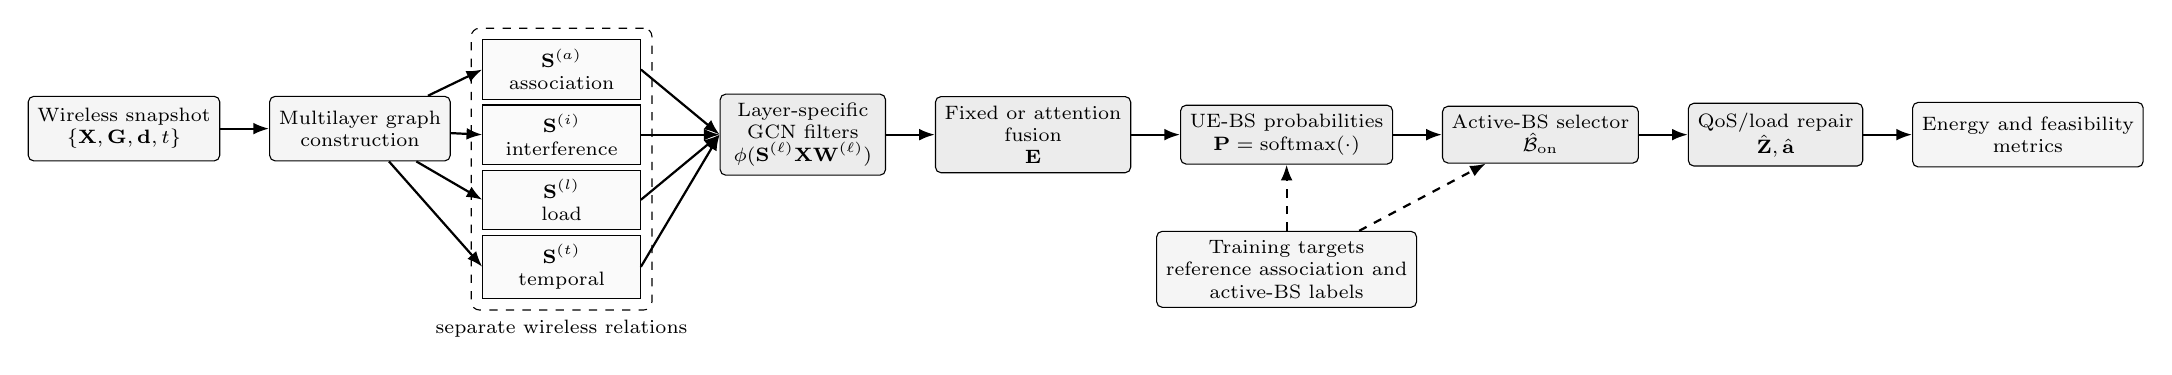
\begin{tikzpicture}[
        font=\scriptsize,
        node distance=0.42cm and 0.62cm,
        block/.style={draw, rounded corners=2pt, align=center,
            minimum height=0.82cm, minimum width=2.25cm, fill=gray!8},
        layer/.style={draw, align=center, minimum height=0.48cm,
            minimum width=2.00cm, fill=gray!4},
        op/.style={draw, rounded corners=2pt, align=center,
            minimum height=0.70cm, minimum width=2.10cm, fill=gray!15},
        arrow/.style={-{Latex[length=2mm]}, thick},
        dashedbox/.style={draw, dashed, rounded corners=3pt, inner sep=4pt}
    ]
    \node[block] (snapshot) {Wireless snapshot\\
    $\{\mathbf{X},\mathbf{G},\mathbf{d},t\}$};
    \node[block, right=of snapshot] (layers) {Multilayer graph\\construction};
    \node[layer, above right=-0.05cm and 0.40cm of layers] (a1)
    {$\mathbf{S}^{(a)}$\\association};
    \node[layer, below=0.06cm of a1] (a2)
    {$\mathbf{S}^{(i)}$\\interference};
    \node[layer, below=0.06cm of a2] (a3)
    {$\mathbf{S}^{(l)}$\\load};
    \node[layer, below=0.06cm of a3] (a4)
    {$\mathbf{S}^{(t)}$\\temporal};
    \node[op, right=1.00cm of a2] (gcn) {Layer-specific\\GCN filters\\
    $\phi(\mathbf{S}^{(\ell)}\mathbf{X}\mathbf{W}^{(\ell)})$};
    \node[op, right=of gcn] (fusion) {Fixed or attention\\fusion\\
    $\mathbf{E}$};
    \node[op, right=of fusion] (prob) {UE-BS probabilities\\
    $\mathbf{P}=\mathrm{softmax}(\cdot)$};
    \node[op, right=of prob] (selector) {Active-BS selector\\
    $\hat{\mathcal{B}}_{\mathrm{on}}$};
    \node[op, right=of selector] (repair) {QoS/load repair\\
    $\hat{\mathbf{Z}},\hat{\mathbf{a}}$};
    \node[block, right=of repair] (metrics) {Energy and feasibility\\
    metrics};

    \draw[arrow] (snapshot) -- (layers);
    \draw[arrow] (layers) -- (a1.west);
    \draw[arrow] (layers) -- (a2.west);
    \draw[arrow] (layers) -- (a3.west);
    \draw[arrow] (layers) -- (a4.west);
    \draw[arrow] (a1.east) -- (gcn.west);
    \draw[arrow] (a2.east) -- (gcn.west);
    \draw[arrow] (a3.east) -- (gcn.west);
    \draw[arrow] (a4.east) -- (gcn.west);
    \draw[arrow] (gcn) -- (fusion);
    \draw[arrow] (fusion) -- (prob);
    \draw[arrow] (prob) -- (selector);
    \draw[arrow] (selector) -- (repair);
    \draw[arrow] (repair) -- (metrics);

    \node[dashedbox, fit=(a1)(a2)(a3)(a4), label=below:{separate wireless relations}] {};
    \node[block, below=0.84cm of prob, minimum width=2.55cm] (train)
    {Training targets\\reference association and\\active-BS labels};
    \draw[arrow, dashed] (train) -- (prob);
    \draw[arrow, dashed] (train) -- (selector);
    \end{tikzpicture}
    }
    \caption{Computational pipeline of the proposed framework. Wireless
    snapshots are converted into separate relation layers, processed by
    layer-specific GCN filters, fused into UE embeddings, and passed to
    association, active-BS selection, repair, and evaluation modules.}
    \label{fig:framework_pipeline}
\end{figure*}


\begin{figure*}[!t]
    \centering
    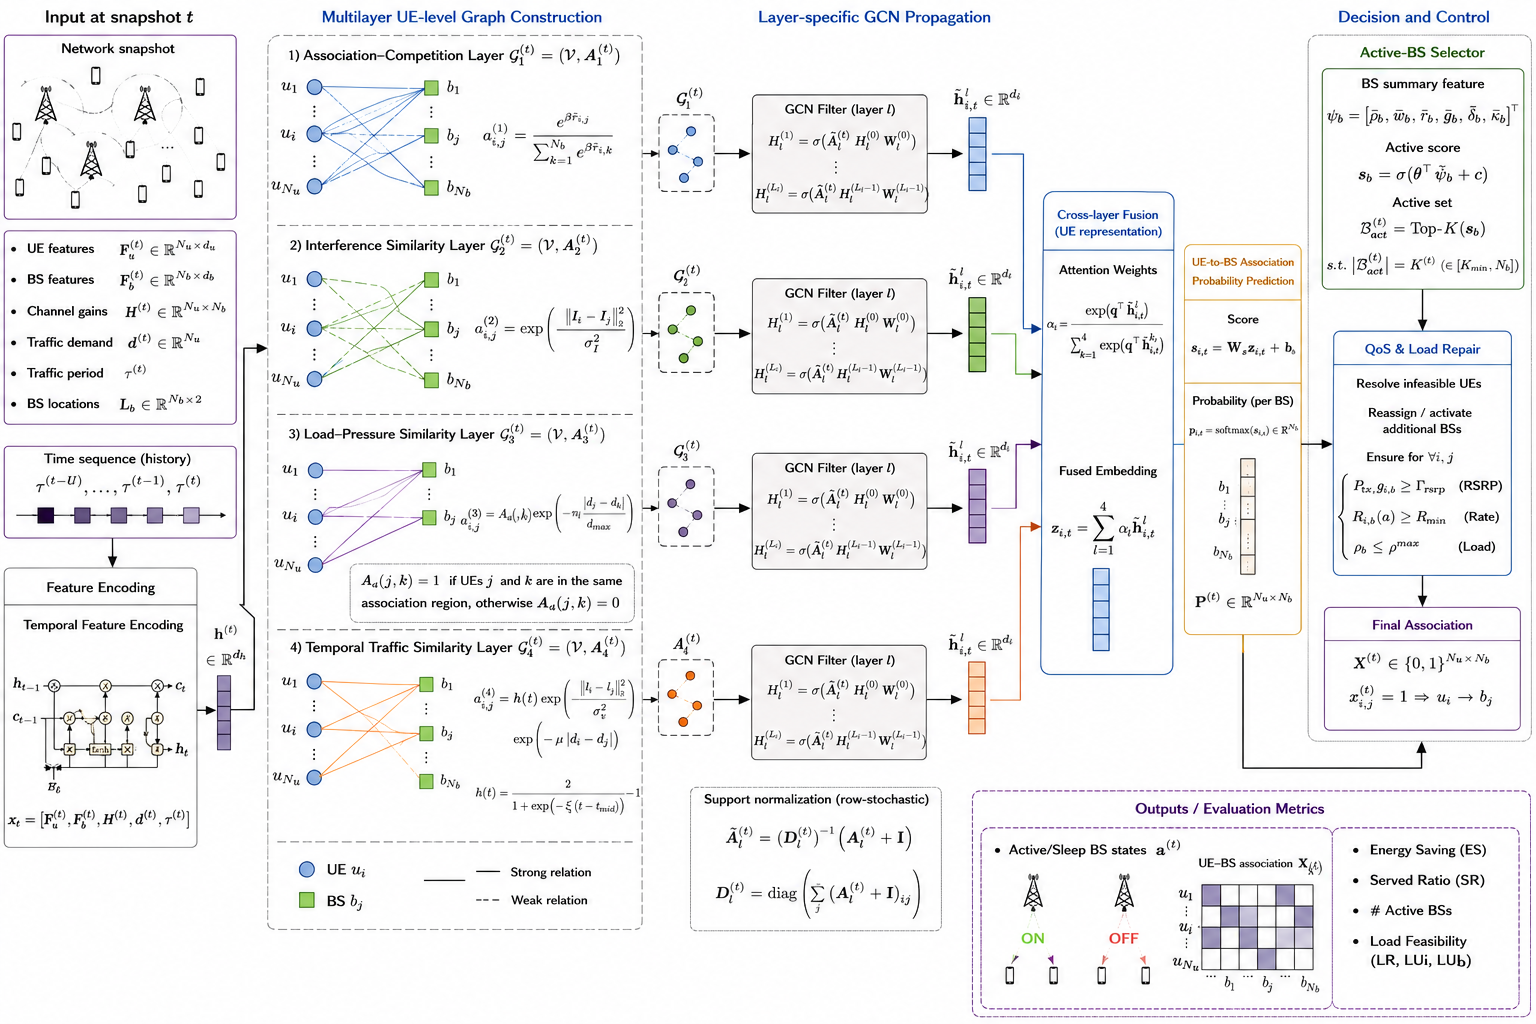
\includegraphics[width=\textwidth]{figures/Model_fig.png}
    \caption{ Proposed multilayer graph-learning framework for energy-aware user association and BS switch-off. At each wireless snapshot, UE features, BS information, channel gains, traffic demand, and temporal context are encoded and used to construct four UE-level wireless relation layers: association-competition, interference-similarity, load-pressure similarity, and temporal-traffic similarity. Each relation layer is processed by a dedicated GCN filter to produce layer-wise UE embeddings, which are then combined through fixed or attention-based cross-layer fusion. The fused UE representation is used to predict UE-to-BS association probabilities, select a compact active-BS set, and apply QoS/load repair and report any residual infeasibility through the served-ratio metric. The final outputs include the UE-BS association matrix, active/sleep BS states, energy saving, served ratio, active-BS count, and load-feasibility metrics.}
    \label{fig:model_architecture}
\end{figure*}

\subsection{Multilayer Wireless Graph Construction}
For each snapshot, let $\mathbf{G}\in\mathbb{R}^{N\times B}$ denote the
channel-gain matrix with entries $g_{i,b}$, and let $\mathbf{r}_i$ be the
position of UE $i$. The proposed model builds a multilayer graph
\begin{equation}
    \mathcal{M} = \left(\mathcal{U},\mathbf{X},
    \{\mathbf{S}^{(\ell)}\}_{\ell\in\mathcal{L}}\right),
    \qquad
    \mathcal{L}=\{a,i,l,t\},
\end{equation}
where $a$, $i$, $l$, and $t$ denote association, interference, load, and
temporal layers, respectively. Each layer is constructed as a nonnegative
adjacency matrix $\mathbf{A}^{(\ell)}$ and converted into a row-stochastic
support matrix
\begin{equation}
    \mathbf{S}^{(\ell)}
    =\left(\mathbf{D}^{(\ell)}\right)^{-1}
    \left(\mathbf{A}^{(\ell)}+\mathbf{I}\right),
    \label{eq:support}
\end{equation}
where $\mathbf{D}^{(\ell)}$ is the diagonal row-sum matrix of
$\mathbf{A}^{(\ell)}+\mathbf{I}$. The identity term preserves each UE's own
features during propagation.

The association layer connects UEs that compete for the same strongest BS. Let
\begin{equation}
    b_i^{\star}=\arg\max_{b\in\mathcal{B}} g_{i,b}.
\end{equation}
Then
\begin{equation}
    A_{j,k}^{(a)} =
    \mathbf{1}\{b_j^{\star}=b_k^{\star}\},
    \qquad j\neq k.
\end{equation}
The interference layer compares normalized channel-gain profiles. Define
$\mathbf{q}_j=\mathbf{g}_j/\|\mathbf{g}_j\|_1$, where $\mathbf{g}_j$ is the
$j$th row of $\mathbf{G}$. The interference similarity is
\begin{equation}
    A_{j,k}^{(i)} = \mathbf{q}_j^T\mathbf{q}_k,\qquad j\neq k.
\end{equation}
The load layer links UEs with similar traffic demand within the same
association region:
\begin{equation}
    A_{j,k}^{(l)} =
    A_{j,k}^{(a)}
    \exp\left(-\eta_l\frac{|d_j-d_k|}{d_{\max}}\right),
\end{equation}
where $\eta_l>0$ controls demand-similarity sharpness and $d_{\max}$ is the
maximum demand scale. Finally, the temporal layer captures spatial-demand
similarity modulated by the traffic period:
\begin{equation}
    A_{j,k}^{(t)} =
    h(t)\exp\left(-\eta_r\frac{\|\mathbf{r}_j-\mathbf{r}_k\|_2}{R}\right)
    \exp\left(-\eta_d\frac{|d_j-d_k|}{d_{\max}}\right),
\end{equation}
where $R$ is the cell-area radius and $h(t)$ is a bounded periodic traffic
factor. Sparse top-$K$ thresholding is applied to the similarity layers to
avoid dense message passing and to emphasize dominant local dependencies.

\subsection{Layer-Aware Association Learning}
Given $\mathbf{X}$ and the supports $\{\mathbf{S}^{(\ell)}\}$, the fixed-fusion
multilayer GCN computes one hidden representation per layer:
\begin{equation}
    \mathbf{H}^{(\ell)}
    =\phi\left(\mathbf{S}^{(\ell)}\mathbf{X}\mathbf{W}^{(\ell)}\right),
    \qquad \ell\in\mathcal{L},
    \label{eq:layer_gcn}
\end{equation}
where $\phi(\cdot)$ is a pointwise nonlinearity and
$\mathbf{W}^{(\ell)}$ is a layer-specific trainable matrix. The layer-wise
embeddings are fused as
\begin{equation}
    \mathbf{E} =
    \left[\mathbf{H}^{(a)}\Vert\mathbf{H}^{(i)}
    \Vert\mathbf{H}^{(l)}\Vert\mathbf{H}^{(t)}\right],
    \label{eq:fixed_fusion}
\end{equation}
where $\Vert$ denotes feature concatenation. The UE-to-BS association
probability matrix is
\begin{equation}
    \mathbf{P} =
    \mathrm{softmax}\left(\mathbf{E}\mathbf{W}_o+\mathbf{b}_o\right),
    \label{eq:association_prob}
\end{equation}
where $P_{i,b}$ is the learned probability that UE $i$ should be associated
with BS $b$.

The attention-weighted model assigns a trainable nonnegative importance weight
to each layer. Let $\eta_{\ell}$ be the attention logit of layer $\ell$. The
normalized layer weight is
\begin{equation}
    \alpha_{\ell} =
    \frac{\exp(\eta_{\ell})}
    {\sum_{r\in\mathcal{L}}\exp(\eta_r)}.
    \label{eq:attention_weight}
\end{equation}
The fused embedding becomes
\begin{equation}
    \mathbf{E}_{\mathrm{att}} =
    \left[|\mathcal{L}|\alpha_a\mathbf{H}^{(a)}
    \Vert |\mathcal{L}|\alpha_i\mathbf{H}^{(i)}
    \Vert |\mathcal{L}|\alpha_l\mathbf{H}^{(l)}
    \Vert |\mathcal{L}|\alpha_t\mathbf{H}^{(t)}\right].
    \label{eq:att_fusion}
\end{equation}
The factor $|\mathcal{L}|$ keeps the scale comparable to fixed fusion when the
attention distribution is uniform.

The association predictor is trained by supervised imitation of low-energy
reference decisions:
\begin{equation}
    \mathcal{L}_{\mathrm{ua}} =
    -\frac{1}{N}\sum_{i\in\mathcal{U}}
    \sum_{b\in\mathcal{B}} y_{i,b}\log P_{i,b},
    \label{eq:ua_loss}
\end{equation}
where $y_{i,b}$ is the reference association label. This loss trains the GNN to
learn association preferences; feasibility and switch-off behavior are handled
by the active-cell and repair stages below.

\subsection{Active-BS Selection and QoS/Load Repair}
Association probabilities alone do not determine which BSs should remain
active, because a model may assign every UE while still keeping unnecessary BSs
on. Therefore, the proposed framework uses a second-stage active-BS selector.
For each BS $b$, a summary vector $\boldsymbol{\psi}_b$ is formed from
probability statistics, demand-weighted probability mass, approximate load,
channel quality, and distance statistics. The active score is
\begin{equation}
    s_b = \sigma\left(\boldsymbol{\theta}^{T}
    \bar{\boldsymbol{\psi}}_b + c\right),
    \label{eq:active_score}
\end{equation}
where $\bar{\boldsymbol{\psi}}_b$ is the standardized BS summary vector and
$\sigma(\cdot)$ is the logistic sigmoid. The selected active set is the set of
top-scoring BSs,
\begin{equation}
    \widehat{\mathcal{B}}_{\mathrm{on}}
    = \operatorname{TopK}_{b\in\mathcal{B}}(s_b).
    \label{eq:topk}
\end{equation}
The value of $K$ is estimated from the average active-BS count of the reference
solutions in the training set.

The initial UE assignment chooses, for each UE, the most likely BS among
$\widehat{\mathcal{B}}_{\mathrm{on}}$. A repair routine then checks the RSRP,
rate, and load constraints in \eqref{eq:rsrp}--\eqref{eq:load_constraint}. If
the selected active set cannot support the snapshot, additional BSs are
activated according to their aggregate gain-demand score over stressed UEs.
Algorithm~\ref{alg:method} gives the complete inference procedure.

\begin{algorithm}[!t]
\caption{Multilayer GNN Association With Active-BS Repair}
\label{alg:method}
\begin{algorithmic}[1]
\Require $(\mathbf{X},\mathbf{G},\mathbf{d},t)$, parameters
$\Theta=\{\mathbf{W}^{(\ell)},\mathbf{W}_o,\mathbf{b}_o,\eta_{\ell}\}$,
selector $(\boldsymbol{\theta},c)$, $K$, fusion mode
$q\in\{\mathrm{fixed},\mathrm{adaptive}\}$
\Ensure $\widehat{\mathbf{Z}}$, $\widehat{\mathbf{a}}$

\State $\mathcal{L}\gets\{a,i,l,t\}$
\State $\mathbf{S}^{(\ell)}\gets\operatorname{LayerSupport}_{\ell}
(\mathbf{X},\mathbf{G},\mathbf{d},t)$, $\ell\in\mathcal{L}$

\For{$\ell\in\mathcal{L}$}
    \State $\mathbf{H}^{(\ell)}
    \gets \phi(\mathbf{S}^{(\ell)}\mathbf{X}\mathbf{W}^{(\ell)})$
\EndFor

\If{$q=\mathrm{fixed}$}
    \State $\mathbf{E}\gets
    \mathbf{H}^{(a)}\Vert \mathbf{H}^{(i)}
    \Vert \mathbf{H}^{(l)}\Vert \mathbf{H}^{(t)}$
\Else
    \State $\alpha_{\ell}\gets
    \exp(\eta_{\ell})/\sum_{r\in\mathcal{L}}\exp(\eta_r)$,
    $\ell\in\mathcal{L}$
    \State $\mathbf{E}\gets
    \Vert_{\ell\in\mathcal{L}}\left(|\mathcal{L}|\alpha_{\ell}
    \mathbf{H}^{(\ell)}\right)$
\EndIf

\State $\mathbf{P}\gets
\operatorname{softmax}(\mathbf{E}\mathbf{W}_o+\mathbf{b}_o)$

\For{$b\in\mathcal{B}$}
    \State $\boldsymbol{\psi}_b\gets\operatorname{BSFeatures}(b,\mathbf{P},
    \mathbf{G},\mathbf{d})$
    \State $s_b\gets\sigma(\boldsymbol{\theta}^{T}\boldsymbol{\psi}_b+c)$
\EndFor

\State $\mathcal{A}\gets\operatorname{TopK}_{b\in\mathcal{B}}(s_b,K)$

\Repeat
    \State $z_{i,b}\gets0$, $\forall i,b$

    \For{$i\in\mathcal{U}$}
        \State $\mathcal{C}_i\gets
        \{b\in\mathcal{A}:R_{i,b}(\mathcal{A})\geq R_{\min},
        P_{\mathrm{tx}}g_{i,b}\geq\Gamma_{\mathrm{rsrp}}\}$

        \If{$\mathcal{C}_i=\varnothing$}
            \State $\mathcal{C}_i\gets\mathcal{A}$
        \EndIf

        \State $b_i\gets\arg\max_{b\in\mathcal{C}_i}P_{i,b}$
        \State $z_{i,b_i}\gets1$
    \EndFor

    \State $\rho_b\gets
    \sum_{i\in\mathcal{U}}z_{i,b}d_i/R_{i,b}(\mathcal{A})$

    \State $\mathcal{V}\gets
    \{i:R_{i,b_i}<R_{\min}\ \text{or}\
    P_{\mathrm{tx}}g_{i,b_i}<\Gamma_{\mathrm{rsrp}}\ \text{or}\
    \rho_{b_i}>\rho_{\max}\}$

    \If{$\mathcal{V}=\varnothing$ or $|\mathcal{A}|=B$}
        \State \textbf{break}
    \EndIf

    \State $b^{+}\gets
    \arg\max_{b\in\mathcal{B}\setminus\mathcal{A}}
    \sum_{i\in\mathcal{V}}d_i g_{i,b}$

    \State $\mathcal{A}\gets\mathcal{A}\cup\{b^{+}\}$

\Until{$\mathcal{V}=\varnothing$ or $|\mathcal{A}|=B$}

\State $\widehat{a}_b\gets\mathbf{1}\{b\in\mathcal{A}\}$, $\forall b$
\State $\widehat{z}_{i,b}\gets z_{i,b}$, $\forall i,b$

\State \Return $\widehat{\mathbf{Z}}$, $\widehat{\mathbf{a}}$
\end{algorithmic}
\end{algorithm}

\subsection{Mathematical Properties}
Let $\mathfrak{M}=(\mathbf{X},\{\mathbf{S}^{(\ell)}\}_{\ell\in\mathcal{L}})$
denote the multilayer input and define the layer-aware encoder
$F_{\Theta}$ by \eqref{eq:layer_gcn}--\eqref{eq:att_fusion}. For a permutation
matrix $\boldsymbol{\Pi}$, define the action
\begin{equation}
    T_{\boldsymbol{\Pi}}(\mathfrak{M}) =
    \left(\boldsymbol{\Pi}\mathbf{X},
    \{\boldsymbol{\Pi}\mathbf{S}^{(\ell)}
    \boldsymbol{\Pi}^{T}\}_{\ell\in\mathcal{L}}\right).
\end{equation}
Define also the feasibility predicate
\begin{equation}
\begin{split}
    \Phi(\mathbf{Z},\mathbf{a})=1
    \Longleftrightarrow\;&
    \eqref{eq:association_constraint},\eqref{eq:active_constraint},
    \eqref{eq:rsrp},\eqref{eq:qos},\eqref{eq:load_constraint}\\
    &\text{hold for }(\mathbf{Z},\mathbf{a}).
\end{split}
\end{equation}

\begin{theorem}[Equivariance of the multilayer encoder]
For any permutation matrix $\boldsymbol{\Pi}$,
\begin{equation}
    F_{\Theta}\left(T_{\boldsymbol{\Pi}}(\mathfrak{M})\right)
    =\boldsymbol{\Pi}F_{\Theta}(\mathfrak{M}).
    \label{eq:equivariance_result}
\end{equation}
\end{theorem}
\begin{IEEEproof}
Let $\mathbf{H}^{(\ell)}$ and $\widetilde{\mathbf{H}}^{(\ell)}$ be the
layer-$\ell$ hidden matrices generated from $\mathfrak{M}$ and
$T_{\boldsymbol{\Pi}}(\mathfrak{M})$, respectively. Then
\begin{equation}
\begin{split}
\widetilde{\mathbf{H}}^{(\ell)}
&=\phi\left(\boldsymbol{\Pi}\mathbf{S}^{(\ell)}
\boldsymbol{\Pi}^{T}\boldsymbol{\Pi}\mathbf{X}\mathbf{W}^{(\ell)}\right)\\
&=\phi\left(\boldsymbol{\Pi}\mathbf{S}^{(\ell)}
\mathbf{X}\mathbf{W}^{(\ell)}\right)
=\boldsymbol{\Pi}\phi\left(\mathbf{S}^{(\ell)}
\mathbf{X}\mathbf{W}^{(\ell)}\right)\\
&=\boldsymbol{\Pi}\mathbf{H}^{(\ell)}.
\end{split}
\end{equation}
Since concatenation and multiplication by scalar $\alpha_{\ell}$ act on feature
coordinates and not on UE indices,
\begin{equation}
\Vert_{\ell\in\mathcal{L}}\alpha_{\ell}
\widetilde{\mathbf{H}}^{(\ell)}
=\boldsymbol{\Pi}\left(
\Vert_{\ell\in\mathcal{L}}\alpha_{\ell}\mathbf{H}^{(\ell)}\right).
\end{equation}
This proves \eqref{eq:equivariance_result}.
\end{IEEEproof}

\begin{theorem}[Non-injectivity of uniform layer aggregation]
Let
\begin{equation}
    C(\mathfrak{M})
    =\left(\mathbf{X},
    \bar{\mathbf{S}}\right),\qquad
    \bar{\mathbf{S}}=\frac{1}{|\mathcal{L}|}
    \sum_{\ell\in\mathcal{L}}\mathbf{S}^{(\ell)},
\end{equation}
be the uniform layer aggregation map. If $|\mathcal{L}|\geq2$, then $C$ is not
injective. Hence any predictor $H(C(\mathfrak{M}))$ cannot distinguish all
multilayer inputs.
\end{theorem}
\begin{IEEEproof}
It is sufficient to construct two distinct inputs with the same image under
$C$. Consider two layers $p$ and $q$, and let $\mathbf{A}\neq\mathbf{B}$.
Define
\begin{equation}
\begin{array}{ll}
\mathfrak{M}_1:\quad
\mathbf{S}^{(p)}=\mathbf{A},\quad
\mathbf{S}^{(q)}=\mathbf{B},\\[2mm]
\mathfrak{M}_2:\quad
\mathbf{S}^{(p)}=\mathbf{B},\quad
\mathbf{S}^{(q)}=\mathbf{A},
\end{array}
\end{equation}
with all remaining layers and $\mathbf{X}$ identical. Then
\begin{equation}
    C(\mathfrak{M}_1)
    =C(\mathfrak{M}_2),
    \qquad
    \mathfrak{M}_1\neq\mathfrak{M}_2.
\end{equation}
Thus $C$ is non-injective. Consequently, every predictor
that factors through $C$ assigns the same output to
$\mathfrak{M}_1$ and $\mathfrak{M}_2$. In contrast, the layer-aware encoder
contains the ordered terms
$\phi(\mathbf{S}^{(p)}\mathbf{X}\mathbf{W}^{(p)})$ and
$\phi(\mathbf{S}^{(q)}\mathbf{X}\mathbf{W}^{(q)})$; for
$\mathbf{W}^{(p)}\neq\mathbf{W}^{(q)}$, the two constructed inputs need not
have identical embeddings.
\end{IEEEproof}

\begin{lemma}[Attention normalization]
Let $\boldsymbol{\alpha}$ be defined by \eqref{eq:attention_weight}. Then
\begin{equation}
    \boldsymbol{\alpha}\in\Delta^{|\mathcal{L}|-1}
    =\{\mathbf{u}\in\mathbb{R}_{+}^{|\mathcal{L}|}:
    \sum_{\ell\in\mathcal{L}}u_{\ell}=1\}.
\end{equation}
\end{lemma}
\begin{IEEEproof}
For all $\ell$, $\exp(\eta_{\ell})>0$; therefore $\alpha_{\ell}\geq0$.
Moreover,
\begin{equation}
    \sum_{\ell\in\mathcal{L}}\alpha_{\ell}
    =
    \frac{\sum_{\ell\in\mathcal{L}}\exp(\eta_{\ell})}
    {\sum_{r\in\mathcal{L}}\exp(\eta_r)}
    =1.
\end{equation}
\end{IEEEproof}

\noindent The layer-attention concentration reported in the experiments is
measured by
\begin{equation}
    H_{\alpha}=-\sum_{\ell\in\mathcal{L}}\alpha_{\ell}\log\alpha_{\ell}.
    \label{eq:attention_entropy}
\end{equation}

\begin{theorem}[Finite monotone repair]
Let $\mathcal{A}^{(0)}$ be the active set initialized by
\eqref{eq:topk}. Algorithm~\ref{alg:method} generates a sequence
$\{\mathcal{A}^{(m)}\}_{m\geq0}$ satisfying
\begin{equation}
    \mathcal{A}^{(0)}\subseteq\mathcal{A}^{(1)}
    \subseteq\cdots\subseteq\mathcal{B}.
    \label{eq:monotone_active}
\end{equation}
Moreover, the number of strict expansions is at most $B-|\mathcal{A}^{(0)}|$,
and if the algorithm returns at iteration $m$ with
$\Phi(\widehat{\mathbf{Z}},\widehat{\mathbf{a}})=1$, then
$(\widehat{\mathbf{Z}},\widehat{\mathbf{a}})$ is feasible for
\eqref{eq:objective}.
\end{theorem}
\begin{IEEEproof}
At any infeasible iteration, the update has the form
\begin{equation}
    \mathcal{A}^{(m+1)}
    =
    \mathcal{A}^{(m)}\cup\{b^{+}_m\},\qquad
    b^{+}_m\in\mathcal{B}\setminus\mathcal{A}^{(m)}.
\end{equation}
Therefore \eqref{eq:monotone_active} holds and each strict expansion increases
$|\mathcal{A}^{(m)}|$ by one. Since $|\mathcal{B}|=B$, at most
$B-|\mathcal{A}^{(0)}|$ strict expansions are possible. If the algorithm exits
with $\Phi(\widehat{\mathbf{Z}},\widehat{\mathbf{a}})=1$, then the association,
activation, RSRP, rate, and load constraints hold by the definition of
$\Phi$.
\end{IEEEproof}

\begin{corollary}[Oracle bound]
Let $\mathcal{C}$ be the finite candidate set searched by the oracle and let
$J(\mathbf{Z},\mathbf{a})=P_{\mathrm{net}}(\mathbf{Z},\mathbf{a})$. If
\begin{equation}
    (\mathbf{Z}^{\star},\mathbf{a}^{\star})
    \in\arg\min_{(\mathbf{Z},\mathbf{a})\in\mathcal{C},\ \Phi(\mathbf{Z},\mathbf{a})=1}
    J(\mathbf{Z},\mathbf{a}),
\end{equation}
then for every feasible
$(\mathbf{Z},\mathbf{a})\in\mathcal{C}$,
\begin{equation}
    J(\mathbf{Z}^{\star},\mathbf{a}^{\star})
    \leq J(\mathbf{Z},\mathbf{a}).
\end{equation}
\end{corollary}
\begin{IEEEproof}
The inequality is the defining property of the minimum over the feasible subset
of $\mathcal{C}$.
\end{IEEEproof}

\section{Experimental Design}
\subsection{Simulation Scenario}
The experimental study uses simulated dense downlink cellular snapshots so that
the true channel, traffic, association, load, and energy quantities are
available for controlled comparison. Each snapshot contains $B$ BSs deployed in
a circular service region and $N$ UEs drawn uniformly over the same region. One
BS is placed at the center and the remaining BSs are placed on a ring, producing
a dense small-cell layout with overlapping coverage. UE traffic demands vary
across space and time: each snapshot is assigned a traffic period
$t\in\{0,\ldots,T-1\}$, and the demand distribution combines lognormal user
variation, a periodic traffic factor, and a spatial hotspot.

The downlink channel gain $g_{i,b}$ includes distance-dependent path loss,
lognormal shadowing, and small-scale fading. Unless otherwise stated, all BSs
transmit with the same power and share the same bandwidth. The all-on network
is used only as a reference operating point; learned and heuristic policies are
allowed to switch off BSs through the active-BS vector $\mathbf{a}$ defined in
Section III. Fig.~\ref{fig:simulation_scenario} illustrates the simulated
deployment and the information flow from snapshot inputs to radio-channel
generation, multilayer graph construction, and control evaluation.
Table~\ref{tab:sim_params} lists the baseline simulation configuration used
for the initial comparative study.

\begin{figure}[!t]
    \centering
    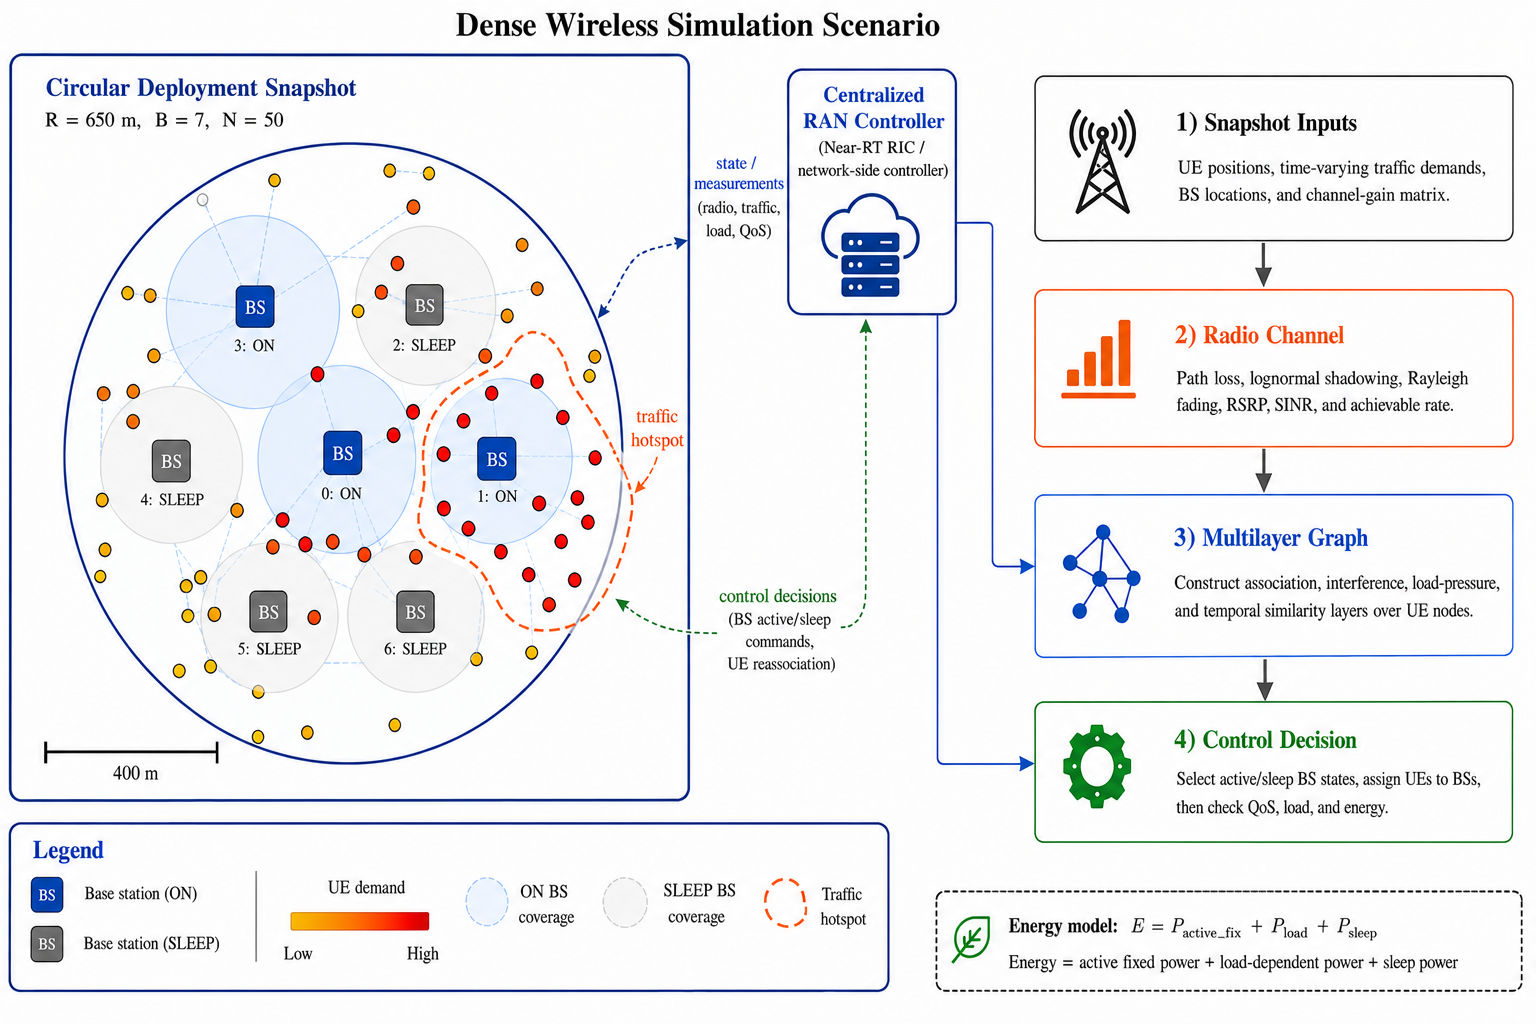
\includegraphics[width=\columnwidth]{figures/Simulation_Scenario_Con.png}
    \caption{Illustrative dense wireless control scenario considered in this
    study. A network-side controller collects radio, traffic, and load
    information from a dense BS cluster, constructs the multilayer UE graph,
    and jointly determines UE association and BS active/sleep states. When a BS
    is switched to sleep mode, its UEs are reassociated to feasible neighboring
    active BSs subject to QoS and load constraints. The scenario is motivated
    by HetNet BS switch-off and load-transfer models in~\cite{ghazzai2017green,oh2013dynamic}
    and by network-side energy-saving control concepts in O-RAN~\cite{oran2025energy}.}
    \label{fig:simulation_scenario}
\end{figure}

\begin{table}[!t]
\caption{Baseline Simulation and Training Configuration}
\label{tab:sim_params}
\centering
\begin{tabular}{ll}
\toprule
Parameter & Value \\
\midrule
Number of BSs, $B$ & 7 \\
Number of UEs, $N$ & 50 \\
Service-region radius & 650 m \\
Carrier frequency & 3.5 GHz \\
Bandwidth & 20 MHz \\
BS transmit power & 20 W \\
Noise power & $-94$ dBm \\
Path-loss exponent & 3.2 \\
Shadowing standard deviation & 6 dB \\
Minimum RSRP threshold & $-115$ dBm \\
Minimum rate, $R_{\min}$ & 1 Mbps \\
Traffic demand range & 0.5--6 Mbps \\
Load limit, $\rho_{\max}$ & 1.0 \\
BS fixed/dynamic/sleep power & 90 W / 55 W / 8 W \\
BS switching cost, $\kappa$ & 35 W-equivalent per state change \\
Traffic periods, $T$ & 24 \\
Training/test snapshots per seed & 60 / 20 \\
Random seeds & 11, 13, 17, 19, 23, 29, 31, 37, 41, 43 \\
Hidden dimension & 24 \\
Training epochs / patience & 80 / 20 \\
Learning rate & 0.018 \\
\bottomrule
\end{tabular}
\end{table}


\subsection{Reference Decisions}
Each training snapshot is labeled by a finite-search reference policy. The
reference policy enumerates candidate active-BS subsets
$\mathcal{A}\subseteq\mathcal{B}$ and assigns UEs greedily within each subset
using channel quality, demand, and projected load. For each candidate, it
computes an energy-penalized score
\begin{align}
    Q(\mathbf{Z},\mathbf{a})
    =&\ P_{\mathrm{net}}(\mathbf{Z},\mathbf{a})
    +\lambda_s\left(1-\mathrm{SR}(\mathbf{Z},\mathbf{a})\right) \nonumber\\
    &+\lambda_{\rho}
    \left[\max_b \rho_b(\mathbf{Z},\mathbf{a})-\rho_{\max}\right]_+,
    \label{eq:reference_score}
\end{align}
where $[x]_+=\max(x,0)$ and $\mathrm{SR}$ is the served ratio. The reference
decision is the lowest-score feasible candidate in the searched set. This
reference is not used as a claimed globally optimal solution of
\eqref{eq:objective}; it is used as a finite benchmark for supervised
training and for measuring the energy gap of learned policies.

\subsection{Compared Policies}
The comparative study evaluates four groups of policies.

First, conventional association heuristics are included as non-learning
baselines. The RSRP policy assigns each UE to the BS with maximum received
power. The SINR policy assigns each UE to the BS with maximum all-on SINR. The
load-aware policy sequentially assigns high-demand UEs to BSs that minimize
projected load while maintaining radio feasibility when possible. These
heuristics are repaired before evaluation using the same QoS/load guard applied
to learned policies, so the comparison measures the quality of the association
preference rather than failure of a postprocessing step.

Second, explicit sleep-control baselines are included to avoid comparing
against association-only heuristics. RSRP-sleep, SINR-sleep, and load-sleep
start from the corresponding association rule and greedily deactivate BSs when
the resulting repaired association remains feasible and reduces energy.
Greedy-sleep is a more demanding baseline that uses the same energy-aware assignment
rule as the finite-search reference but performs backward one-cell pruning
instead of enumerating all active-BS subsets. These baselines evaluate whether
a learned policy improves over hand-designed BS switch-off logic.

Third, single-representation learning baselines are trained on the same
reference labels. The flat MLP receives UE features only and does not use graph
propagation. The aggregated GCN uses the average support
\begin{equation}
    \bar{\mathbf{S}}=\frac{1}{|\mathcal{L}|}
    \sum_{\ell\in\mathcal{L}}\mathbf{S}^{(\ell)}
\end{equation}
and therefore receives a single graph representation. These two baselines
separate the value of graph propagation from the value of preserving separate
relation layers.

Fourth, the proposed multilayer models are evaluated. The fixed-fusion ML-GCN
uses \eqref{eq:layer_gcn}--\eqref{eq:fixed_fusion}, while the attention ML-GCN
uses \eqref{eq:attention_weight}--\eqref{eq:att_fusion}. For each learned
representation, we report the fixed top-$K$ policy, the score-guided pruned
policy, and the stability-aware pruned policy. A finite-search reference policy
is reported as an upper-bound benchmark within the searched candidate class.

\subsection{Training Protocol}
All learning models are trained by minimizing the association loss in
\eqref{eq:ua_loss} over the training snapshots. Node features are standardized
using the training set statistics and the same transformation is applied to the
test snapshots. The active-BS selector is trained after the association model by
using the model probability outputs and the reference active sets. The number
of selected active BSs is initialized from the rounded mean active-BS count of
the reference decisions in the training set.

For each test snapshot, a learned model first outputs UE-to-BS probabilities,
then active-BS scores, then an initial association over the selected active set.
Algorithm~\ref{alg:method} finally checks RSRP, rate, and load constraints and
activates additional BSs only when the selected set cannot support the
snapshot. All reported metrics are computed after this final repaired decision.

\subsection{Evaluation Metrics}
The primary metric is network energy. Let
$P_{\mathrm{all}}$ denote the energy consumed when all BSs are active under the
same power model. The energy saving of a policy $\pi$ is
\begin{equation}
    \mathrm{ES}_{\pi}
    =
    \frac{P_{\mathrm{all}}-P_{\pi}}{P_{\mathrm{all}}},
    \label{eq:energy_saving_metric}
\end{equation}
where $P_{\pi}=P_{\mathrm{net}}(\mathbf{Z}_{\pi},\mathbf{a}_{\pi})$. The
energy gap relative to the reference policy is
\begin{equation}
    \mathrm{Gap}_{\pi}
    =
    \frac{P_{\pi}-P_{\mathrm{ref}}}{P_{\mathrm{ref}}},
    \label{eq:oracle_gap_metric}
\end{equation}
where $P_{\mathrm{ref}}$ is the reference energy for the same snapshot.

Constraint satisfaction is measured by served ratio,
\begin{align}
    \mathrm{SR}_{\pi}
    =&\ \frac{1}{N}\sum_{i=1}^{N}
    \mathbf{1}\Big\{
    P_{\mathrm{tx}}g_{i,b_i}\geq\Gamma_{\mathrm{rsrp}},
    \nonumber\\
    &\qquad\qquad
    R_{i,b_i}\geq R_{\min},
    \ \rho_{b_i}\leq\rho_{\max}
    \Big\}.
    \label{eq:served_ratio_metric}
\end{align}
Operational compactness and load behavior are reported using active-BS count
\begin{equation}
    A_{\pi}=\sum_{b\in\mathcal{B}}a_{\pi,b},
\end{equation}
maximum load
\begin{equation}
    \rho_{\max}^{\pi}=\max_{b\in\mathcal{B}}\rho_b,
\end{equation}
and mean active load
\begin{equation}
    \bar{\rho}_{\mathrm{on}}^{\pi}
    =
    \frac{\sum_{b\in\mathcal{B}}a_{\pi,b}\rho_b}
    {\sum_{b\in\mathcal{B}}a_{\pi,b}}.
\end{equation}
Assignment accuracy against reference labels is reported only as a diagnostic,
because a policy can have low label agreement while still producing a feasible
low-energy association.

\subsection{Layer Ablation and Stress Tests}
To evaluate the role of each relation layer, the experiments include
single-layer and leave-one-layer-out variants of the ML-GCN. For a layer
$\ell$, the leave-one-layer-out energy effect is
\begin{equation}
    \Delta_{\ell}^{(-)}
    =
    \mathrm{ES}_{\mathrm{full}}
    -
    \mathrm{ES}_{-\ell},
    \label{eq:leave_one_out_metric}
\end{equation}
and the single-layer contribution is
\begin{equation}
    \Delta_{\ell}^{(+)}
    =
    \mathrm{ES}_{\ell}
    -
    \mathrm{ES}_{\mathrm{flat}}.
    \label{eq:single_layer_metric}
\end{equation}
Positive $\Delta_{\ell}^{(-)}$ indicates that removing layer $\ell$ reduces
energy saving, while positive $\Delta_{\ell}^{(+)}$ indicates that layer
$\ell$ alone improves over a feature-only model.

Pairwise layer redundancy is measured before training using support-matrix
dissimilarity,
\begin{equation}
    D_{\ell,r}
    =
    \frac{\|\mathbf{S}^{(\ell)}-\mathbf{S}^{(r)}\|_F}
    {\|\mathbf{S}^{(\ell)}\|_F+\epsilon},
    \qquad \ell\neq r,
    \label{eq:layer_dissimilarity}
\end{equation}
where $\epsilon>0$ avoids division by zero. Attention concentration is measured
using \eqref{eq:attention_entropy}. In addition to the baseline setting in ~\ref{tab:sim_params}, stress tests vary bandwidth, QoS threshold, UE density, and shadowing variance.

\section{Results and Discussion}

\subsection{Static Energy Versus Switching-Aware Control}

Table~\ref{tab:ten_seeds_results} reports the main ten-seed simulation
comparison. The focus is the operational comparison between greedy sleep
control and the proposed stability-aware multilayer graph controllers. Greedy
sleep is a non-learning BS switch-off baseline that directly
removes cells when one-cell pruning reduces snapshot energy. However, the
simulation results show that the proposed stability-aware ML-GCN improves
over greedy sleep under both static and switching-adjusted energy while
preserving full service feasibility.

The stability-aware ML-GCN search policy achieves $79.0\%$ static energy
saving and $76.1\%$ switching-adjusted energy saving relative to the all-on
network. Greedy sleep achieves $76.9\%$ static saving and $68.3\%$
switching-adjusted saving. Thus, the learned multilayer controller reduces
static energy while also reducing the switching penalty caused by active-BS
churn. The improvement is not obtained by relaxing constraints: both
stability-aware ML-GCN search and greedy sleep maintain served ratio $1.0$.
The main operational difference is that stability-aware ML-GCN search uses
fewer BS state transitions, reducing the mean number of state changes from
$2.50$ for greedy sleep to $0.85$ per snapshot.

The finite-search reference is retained as a bounded reference and training
signal. It gives the largest static saving among the searched candidates,
whereas stability-aware ML-GCN search gives the largest switching-adjusted
saving among the implementable policies in this simulation comparison. This
distinction supports the modeling hypothesis: preserving multilayer wireless
structure and applying stability-aware active-cell control can improve
energy-efficient BS switch-off when both static energy and switching behavior
are reported.

\begin{table*}[!t]
\caption{Ten-Seed Performance With Switching Cost}
\label{tab:ten_seeds_results}
\centering
\small
\begin{tabular}{lccccc}
\toprule
Policy & Switching saving & Static saving & Switches & Served ratio & Active BSs \\
\midrule
Reference search & $0.7372\pm0.0121$ & $0.8040\pm0.0050$ & $1.938\pm0.225$ & $1.000$ & $1.279$ \\
ML-GCN-search & $0.7350\pm0.0133$ & $0.8038\pm0.0052$ & $1.996\pm0.253$ & $1.000$ & $1.279$ \\
ML-GCN-stable-search & $0.7610\pm0.0084$ & $0.7905\pm0.0076$ & $0.854\pm0.177$ & $1.000$ & $1.400$ \\
Attn-ML-GCN-stable-search & $0.7610\pm0.0085$ & $0.7904\pm0.0077$ & $0.854\pm0.177$ & $1.000$ & $1.400$ \\
Flat MLP-stable-search & $0.7607\pm0.0086$ & $0.7893\pm0.0097$ & $0.829\pm0.197$ & $1.000$ & $1.408$ \\
Greedy sleep & $0.6828\pm0.0138$ & $0.7692\pm0.0071$ & $2.504\pm0.308$ & $1.000$ & $1.721$ \\
ML-GCN-pruned & $0.7338\pm0.0123$ & $0.7868\pm0.0073$ & $1.538\pm0.256$ & $1.000$ & $1.458$ \\
Attn-ML-GCN-pruned & $0.7338\pm0.0124$ & $0.7869\pm0.0073$ & $1.538\pm0.256$ & $1.000$ & $1.458$ \\
RSRP sleep & $0.6813\pm0.0184$ & $0.7682\pm0.0092$ & $2.521\pm0.279$ & $1.000$ & $1.742$ \\
RSRP & $0.3223\pm0.0034$ & $0.3230\pm0.0035$ & $0.021\pm0.035$ & $1.000$ & $6.988$ \\
\bottomrule
\end{tabular}
\end{table*}

\begin{figure}[!t]
    \centering
    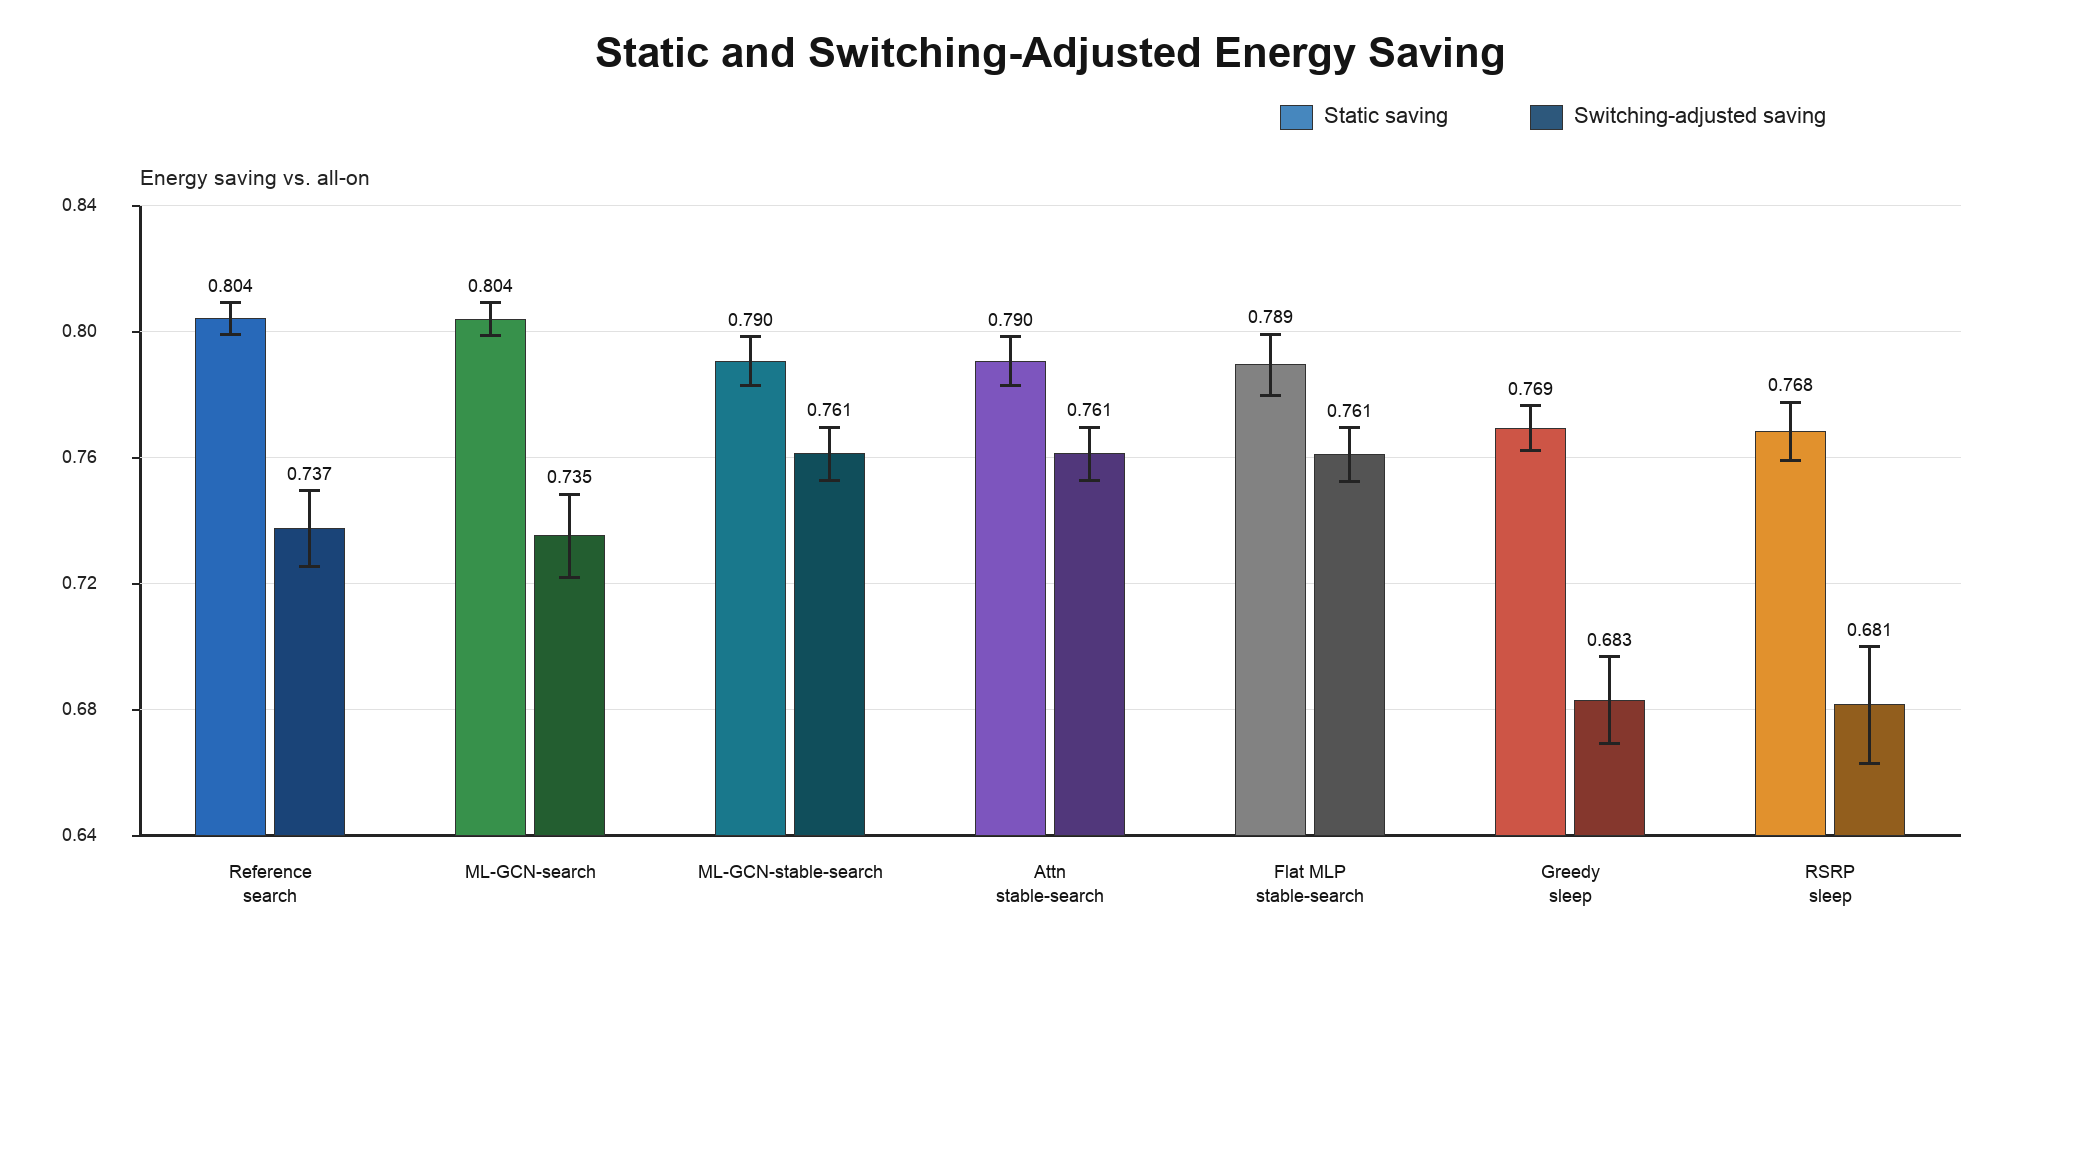
\includegraphics[width=\columnwidth]{figures/results/fig_stable_switching_energy_saving.png}
    \caption{Static and switching-adjusted energy saving across the main
    policies. Stability-aware ML-GCN search has higher saving than greedy sleep under both
    reported energy metrics while preserving full served ratio.}
    \label{fig:stable_energy}
\end{figure}


\subsection{Effect of Stability-Aware Pruning}
Fig.~\ref{fig:stable_switches} reports the BS state-change behavior.
Stability-aware pruning reduces active-cell churn by reusing the previous
active set when it remains feasible and accepting a state change only when the
switching-adjusted objective improves or feasibility requires it. In the
simulation results, ML-GCN-stable-search has fewer mean state changes than
both ML-GCN-pruned and greedy sleep.

Relative to score-guided ML-GCN-pruned, the stable-search version increases
switching-adjusted saving from $73.4\%$ to $76.1\%$ while reducing state
changes from $1.54$ to $0.85$ per snapshot. Relative to greedy sleep,
ML-GCN-stable-search reduces mean state changes by approximately $1.65$ per
snapshot. The reduction is operationally relevant because BS ON/OFF
transitions can incur signaling, hardware, and service-continuity costs. The
result also identifies the role of the decision layer: multilayer graph learning
provides association preferences from heterogeneous wireless relations, while
stability-aware pruning converts those preferences into compact and temporally
smoother active-BS sequences.

\begin{figure}[!t]
    \centering
    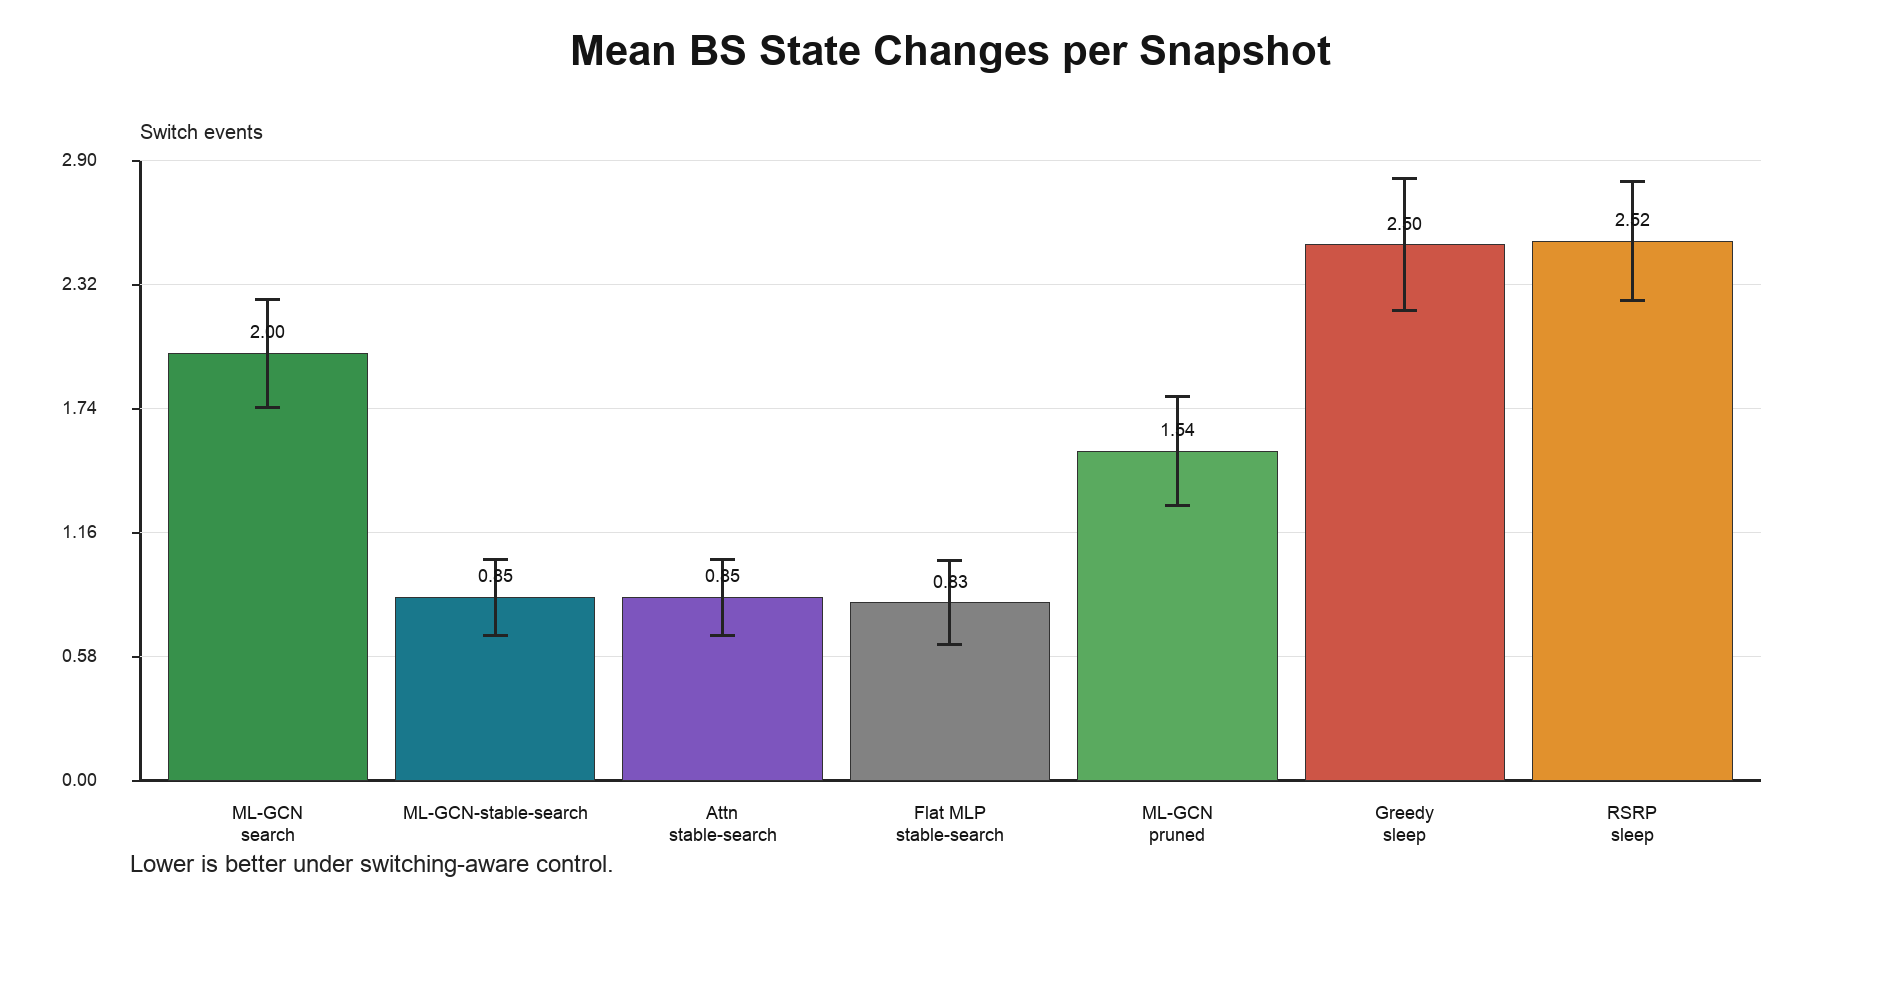
\includegraphics[width=\columnwidth]{figures/results/fig_stable_switch_events.png}
    \caption{Mean BS state changes per snapshot. Stability-aware ML-GCN
    reduces active-cell churn compared with greedy sleep and score-guided
    pruning.}
    \label{fig:stable_switches}
\end{figure}

\subsection{Switching-Cost Sensitivity}
Fig.~\ref{fig:switching_sweep} shows the sensitivity to the BS switching
penalty $\kappa$. When switching is free, policies with aggressive pruning can
perform well because the objective reduces to static snapshot energy. As
$\kappa$ increases, the ranking shifts toward policies that avoid unnecessary
active-cell transitions. Around the operating value $\kappa=35$ W-equivalent
used in the baseline configuration, ML-GCN-stable-search is above greedy sleep
and the other learned baselines under switching-adjusted saving.

This sensitivity analysis evaluates the effect of transition cost on BS
switch-off decisions. A controller that saves static energy by rapidly changing
BS states can lose part of its benefit when switching overhead is included. The
proposed stable-search ML-GCN preserves most of the static energy benefit while
reducing state-change cost, yielding the largest switching-adjusted saving in
the simulation comparison.

\begin{figure}[!t]
    \centering
    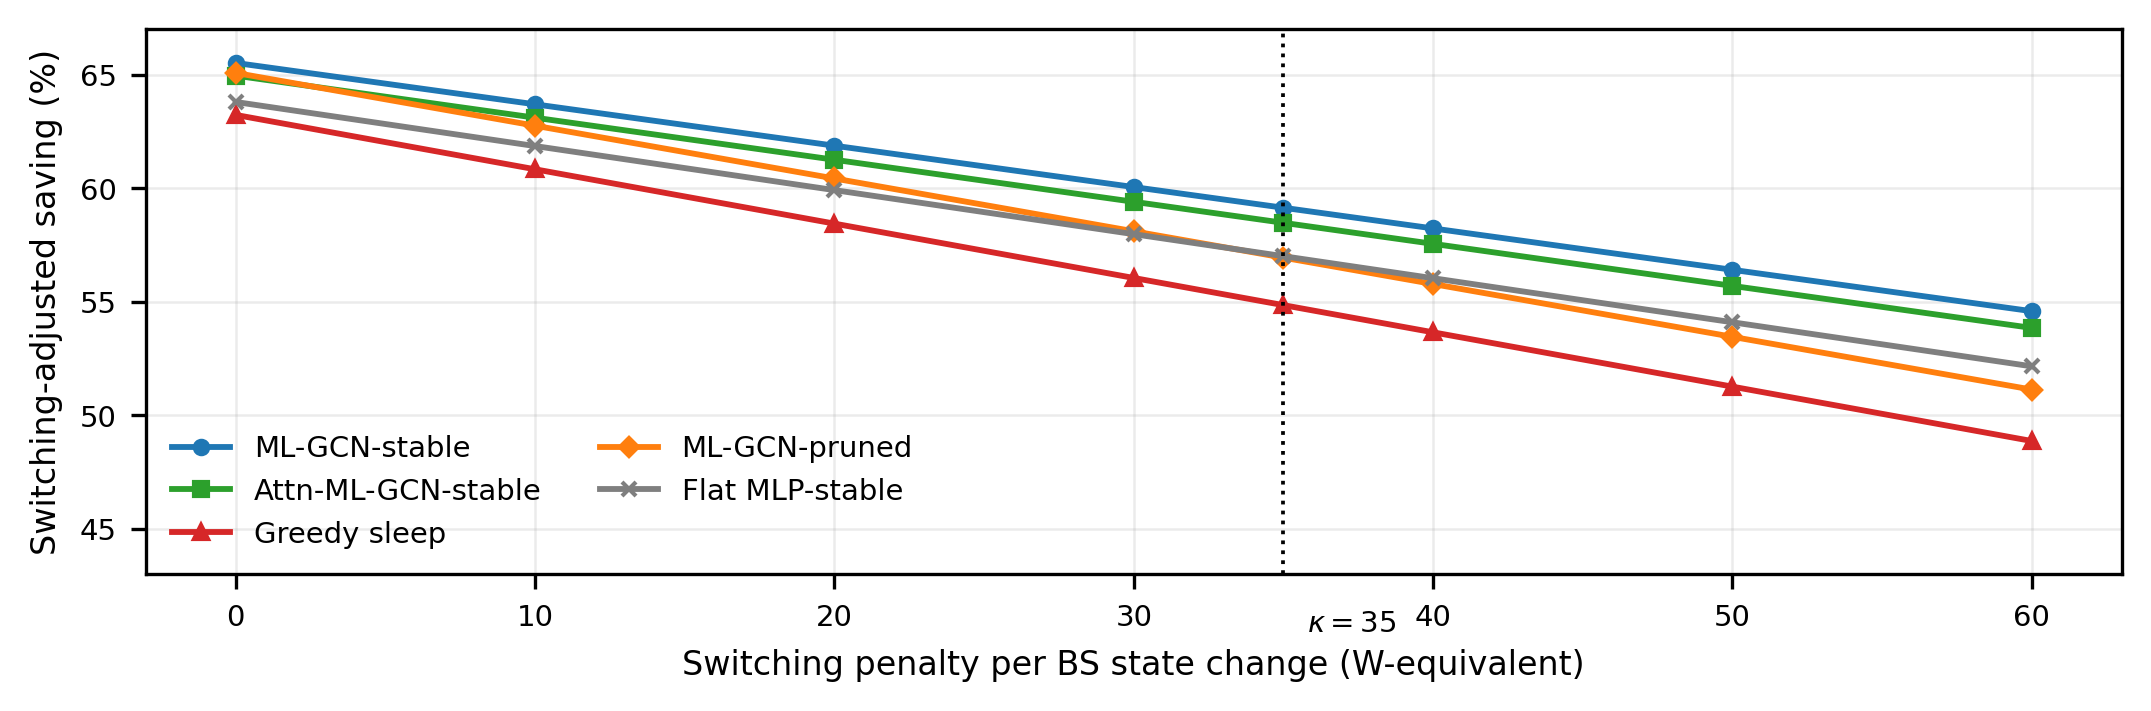
\includegraphics[width=\columnwidth]{figures/results/fig_switching_cost_sweep.png}
    \caption{Sensitivity to the BS switching penalty. Stable multilayer graph
    control provides higher switching-adjusted saving as active-cell
    transitions become costly.}
    \label{fig:switching_sweep}
\end{figure}

\subsection{Multilayer Representation and Learned Baselines}
The results are reported for the complete multilayer graph-control pipeline
rather than for assignment accuracy alone.
The flat MLP uses UE features without graph propagation, while the aggregated
GCN collapses heterogeneous wireless relations into one support. The
multilayer GCN preserves association competition, interference similarity,
load pressure, and temporal traffic similarity as separate relation channels
before active-cell selection and repair.

Table~\ref{tab:component_ablation} separates the effect of representation from
the effect of the active-set decision layer. ML-GCN-search reaches the largest
static saving among learned online policies because it closely follows the
finite-search reference, but it changes BS states more frequently. Adding
stability reduces state changes and improves switching-adjusted saving. The
comparison with Flat MLP-stable-search quantifies the contribution of the
stable active-set controller to switching-aware performance. The multilayer
representation contributes by preserving
relation-aware association preferences and by maintaining comparable performance across the
static, switching, ablation, dissimilarity, and robustness views, rather than
by acting as an isolated classifier.

\begin{table*}[!t]
\caption{Component Ablation: Representation Versus Active-Set Control}
\label{tab:component_ablation}
\centering
\small
\setlength{\tabcolsep}{4pt}
\begin{tabular}{p{0.16\textwidth}p{0.31\textwidth}p{0.13\textwidth}p{0.13\textwidth}p{0.10\textwidth}}
\toprule
Policy & Main component tested & Static saving & Switching saving & Switches \\
\midrule
Greedy sleep & Hand-designed active-cell pruning & $0.7692\pm0.0071$ & $0.6828\pm0.0138$ & $2.504\pm0.308$ \\
ML-GCN-search & Multilayer representation with search, no stability inertia & $0.8038\pm0.0052$ & $0.7350\pm0.0133$ & $1.996\pm0.253$ \\
ML-GCN-stable & Multilayer representation with stability-aware pruning & $0.7857\pm0.0074$ & $0.7469\pm0.0098$ & $1.125\pm0.196$ \\
Flat MLP-stable-search & Feature-only representation with stable search & $0.7893\pm0.0097$ & $0.7607\pm0.0086$ & $0.829\pm0.197$ \\
ML-GCN-stable-search & Multilayer representation with stable search & $0.7905\pm0.0076$ & $0.7610\pm0.0084$ & $0.854\pm0.177$ \\
\bottomrule
\end{tabular}
\end{table*}

The ML-GCN-stable-search policy obtains the largest switching-adjusted saving
among the multilayer policies in the simulation comparison because it combines
three ingredients:
relation-aware association preferences, compact active-BS search, and
switching-aware stability. The pruned ML-GCN has comparable static
saving, but it changes BS states more often than the stable version. The
attention ML-GCN also has comparable performance but remains slightly below the
fixed-fusion ML-GCN in this run, suggesting that the present global attention
mechanism may still be conservative. Snapshot-dependent attention remains a potential
extension.

\subsection{Runtime and Complexity}
Table~\ref{tab:runtime_complexity} reports CPU timing and online decision
complexity for the revised policies. The benchmark uses $N=50$ UEs, $B=7$ BSs,
12 training snapshots, and 5 test snapshots for timing. Let $L$ denote the
number of relation layers, $d$ the input feature dimension, $h$ the hidden
dimension, and $R$ the cost of one repair/evaluation pass. Offline training is
reported separately because it is amortized before deployment.

\begin{table*}[!t]
\caption{Runtime and Online Complexity Benchmark}
\label{tab:runtime_complexity}
\centering
\small
\begin{tabular}{lccc}
\toprule
Policy & Offline fit (s) & Median latency (ms) & Online decision complexity \\
\midrule
RSRP & -- & 3.48 & $\mathcal{O}(NB)$ \\
Load-aware & -- & 5.13 & $\mathcal{O}(NB+N\log N)$ \\
Load-sleep & -- & 36.16 & $\mathcal{O}(B^{2}N+B N\log N)$ \\
Greedy sleep & -- & 84.17 & $\mathcal{O}(B^{2}N+B N\log N)$ \\
ML-GCN & 0.21 & 4.98 & $\mathcal{O}(\sum_{\ell}|E_{\ell}|d+LNdh+LNhB)$ \\
ML-GCN-pruned & 0.21 & 40.06 & $\mathcal{O}(\sum_{\ell}|E_{\ell}|d+LNdh+LNhB+BR)$ \\
ML-GCN-stable & 0.21 & 51.50 & $\mathcal{O}(\sum_{\ell}|E_{\ell}|d+LNdh+LNhB+BR)$ \\
Attn-ML-GCN-stable & 0.31 & 41.20 & $\mathcal{O}(\sum_{\ell}|E_{\ell}|d+LNdh+LNhB+BR)$ \\
Reference search & -- & 228.75 & $\mathcal{O}(2^{B}NB)$ \\
\bottomrule
\end{tabular}
\end{table*}

The runtime results support the switching-aware comparison. Greedy sleep is a
hand-designed controller, but its online latency is higher than
ML-GCN-stable and attention-ML-GCN-stable in the timing benchmark. The
finite-search reference is slower and scales exponentially with
$B$; it is therefore used as a bounded reference and training signal rather
than as an online controller. The stable learned policies therefore provide an
intermediate operating point: they have fewer BS state changes than greedy
sleep under switching cost and lower inference latency than greedy sleep and
finite search in the timing benchmark.

\subsection{Representative Snapshot Behavior}
Fig.~\ref{fig:results_snapshot} shows one representative test snapshot. The
left panel gives the all-on SINR matrix, sorted by the reference association.
The center and right panels compare the reference association and the ML-GCN
association on the same UE/BS geometry. Both decisions preserve full service,
but the learned policy uses one additional active BS in this snapshot. This is
consistent with the aggregate results: the learned controller approaches the
reference switch-off behavior but remains more conservative in order to satisfy
QoS and load constraints after repair.

The snapshot also illustrates why assignment accuracy is not sufficient as a
primary metric. A UE can be moved from one feasible BS to another and still
produce a valid low-energy decision. Therefore, the correct evaluation target
is not exact label reproduction; it is constrained network control measured by
energy, active BS count, load, and served ratio.

\begin{figure}[!t]
    \centering
    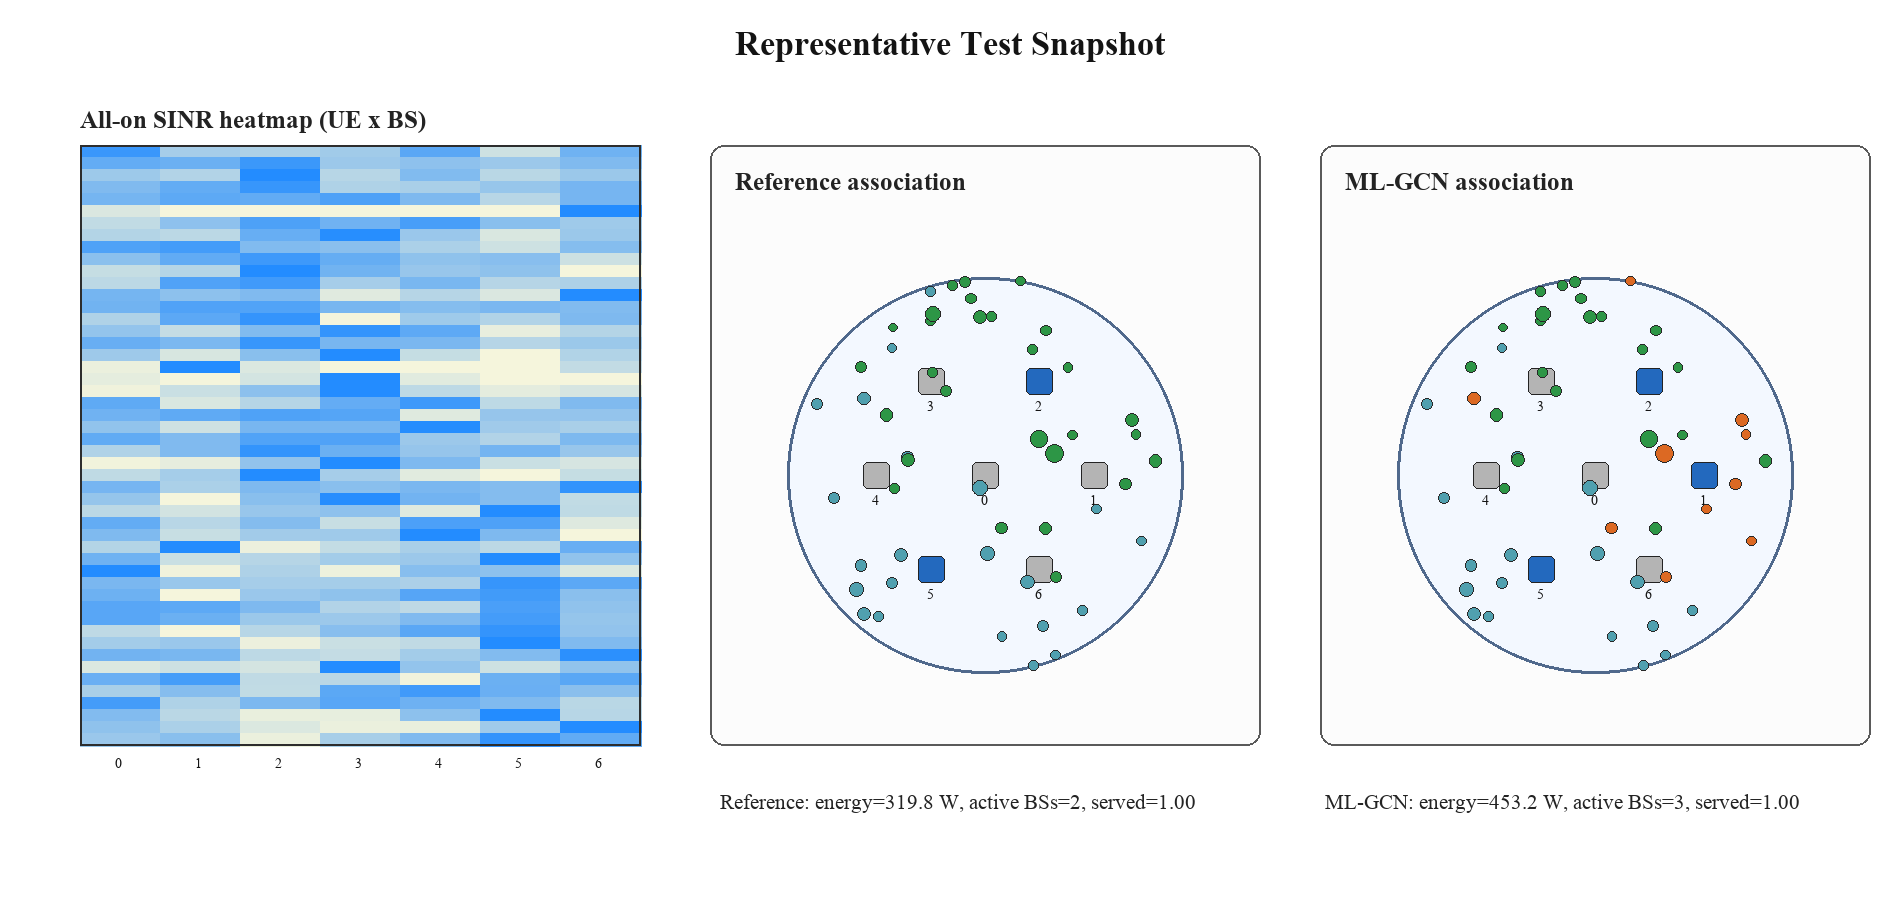
\includegraphics[width=\columnwidth]{figures/results/fig_results_representative_snapshot.png}
    \caption{Representative test snapshot. The heatmap shows all-on SINR over
    UE-BS pairs; the association maps show the finite-search reference and the
    ML-GCN decision after QoS/load repair. The learned policy maintains full
    service while selecting a compact active-BS set.}
    \label{fig:results_snapshot}
\end{figure}

\subsection{Bandwidth and QoS Sensitivity}
Fig.~\ref{fig:results_bandwidth_qos} evaluates bandwidth and QoS sensitivity.
At 10 MHz, the network is highly resource constrained; all methods show low
served ratio and energy saving is limited because most BSs must remain active.
As bandwidth increases, the reference and learned policies exploit the
additional capacity by switching off more BSs. At 20 MHz, ML-GCN reaches
$51.5\%$ energy saving with full served ratio, while RSRP and load-aware
association remain near $17\%$ because they do not actively compact the BS set.
At 80 MHz, the learned controllers exceed $80\%$ energy saving and approach the
reference trend.

The QoS sweep is comparatively flat under the tested range
$R_{\min}\in[0.5,2]$ Mbps. This indicates that, in the baseline traffic and
bandwidth setting, the dominant limiting factor is not the minimum-rate
threshold itself but the load and active-cell structure created by the
association policy. More aggressive QoS stress would require higher demand or
lower bandwidth if rate feasibility is to become the dominant bottleneck.

\begin{figure}[!t]
    \centering
    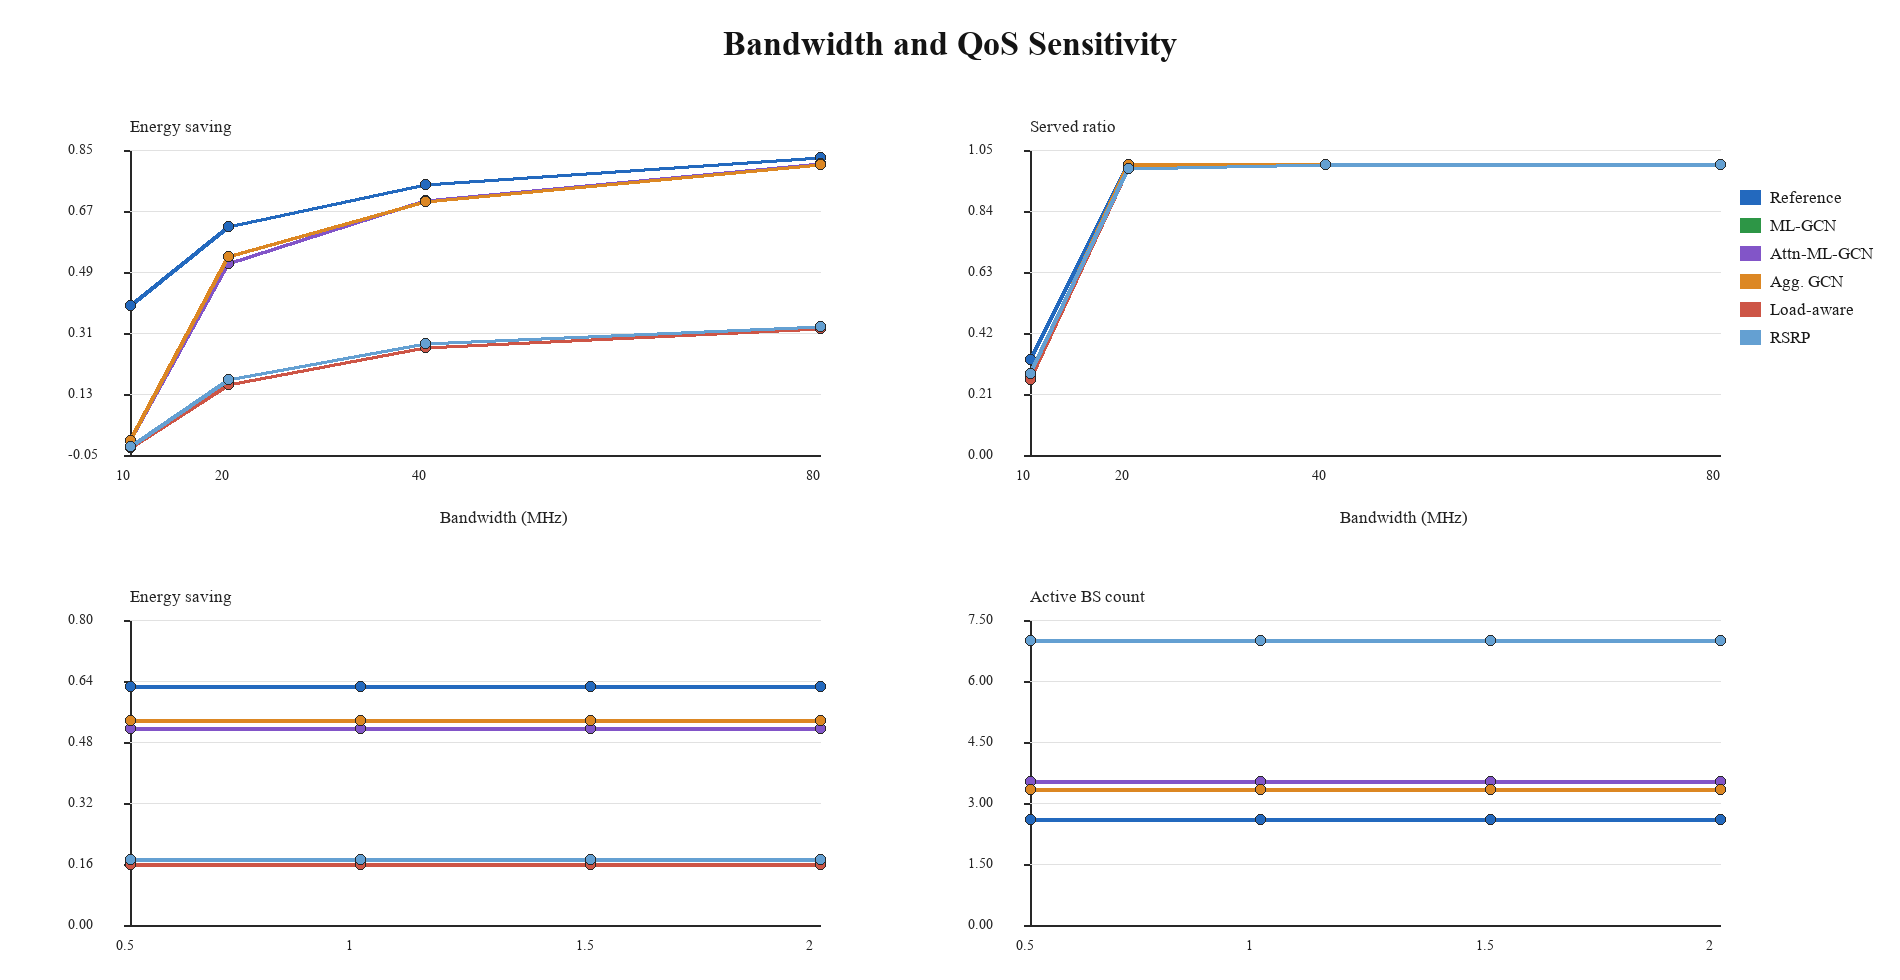
\includegraphics[width=\columnwidth]{figures/results/fig_results_bandwidth_qos.png}
    \caption{Bandwidth and QoS sensitivity. Increasing bandwidth creates
    additional opportunity for BS switch-off, while the tested QoS range is not
    the dominant limiting factor under the baseline traffic load.}
    \label{fig:results_bandwidth_qos}
\end{figure}

To complement the one-dimensional sweeps, Fig.~\ref{fig:results_surface}
reports a joint QoS-density stress surface for ML-GCN under three shadowing
levels. The surface confirms that UE density is the dominant stressor in the
tested regime: energy saving remains high when the network has 30--50 UEs, but
decreases sharply as the UE count grows to 70--90. Changes in the QoS threshold
produce a smaller effect than density, which is consistent with the earlier QoS
sweep. This behavior indicates that the learned controller is mainly limited by
load concentration and active-cell capacity under dense traffic, rather than by
the minimum-rate threshold alone.

\begin{figure}[!t]
\centering
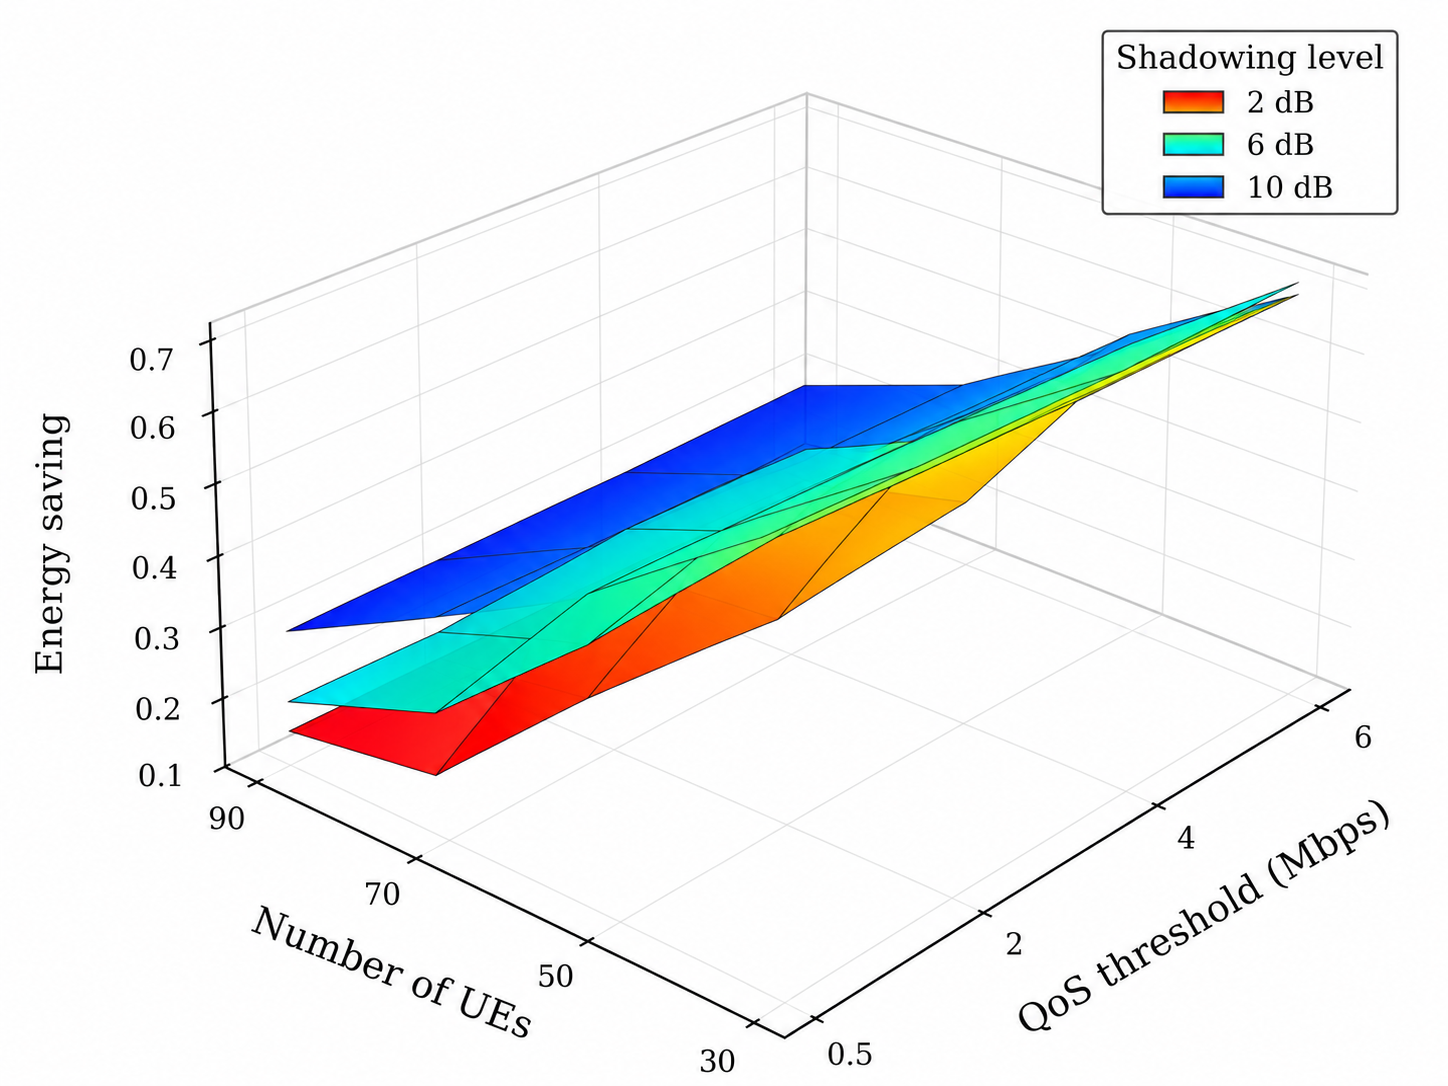
\includegraphics[width=0.9\columnwidth]{figures/results/fig_results_surface_energy.png}
\caption{Joint QoS-density surface for the proposed ML-GCN. Each surface
reports mean energy saving after QoS/load repair for a different shadowing
standard deviation. UE density has a larger effect on energy saving than the
tested QoS-threshold variation.}
\label{fig:results_surface}
\end{figure}

\subsection{Scalability and Channel Robustness}
Fig.~\ref{fig:results_scalability} studies UE-density and shadowing sweeps. As
the number of UEs increases from 30 to 90, all policies experience reduced
energy saving because additional traffic requires more active BSs. The
reference decreases from $73.8\%$ to $39.2\%$ energy saving, while ML-GCN
decreases from $70.5\%$ to $20.6\%$. The gap widens in the dense-load regime,
which suggests that the current learned active-BS selector is conservative when
many UEs compete for limited resources. Nevertheless, ML-GCN remains above RSRP
and load-aware association across the density sweep.

The shadowing sweep shows that the learned policies are stable under channel
uncertainty in the tested range. ML-GCN maintains full served ratio and
approximately $51$--$55\%$ energy saving as the shadowing standard deviation
varies from 2 to 14 dB. The reference energy saving also remains close to
$62$--$63\%$. This robustness is expected because the multilayer representation
uses multiple relational views: channel-profile similarity, association
competition, demand/load structure, and temporal similarity. If one view becomes
noisier, the remaining layers still provide discriminative structure for active-cell
selection and association repair.

\begin{figure}[!t]
    \centering
    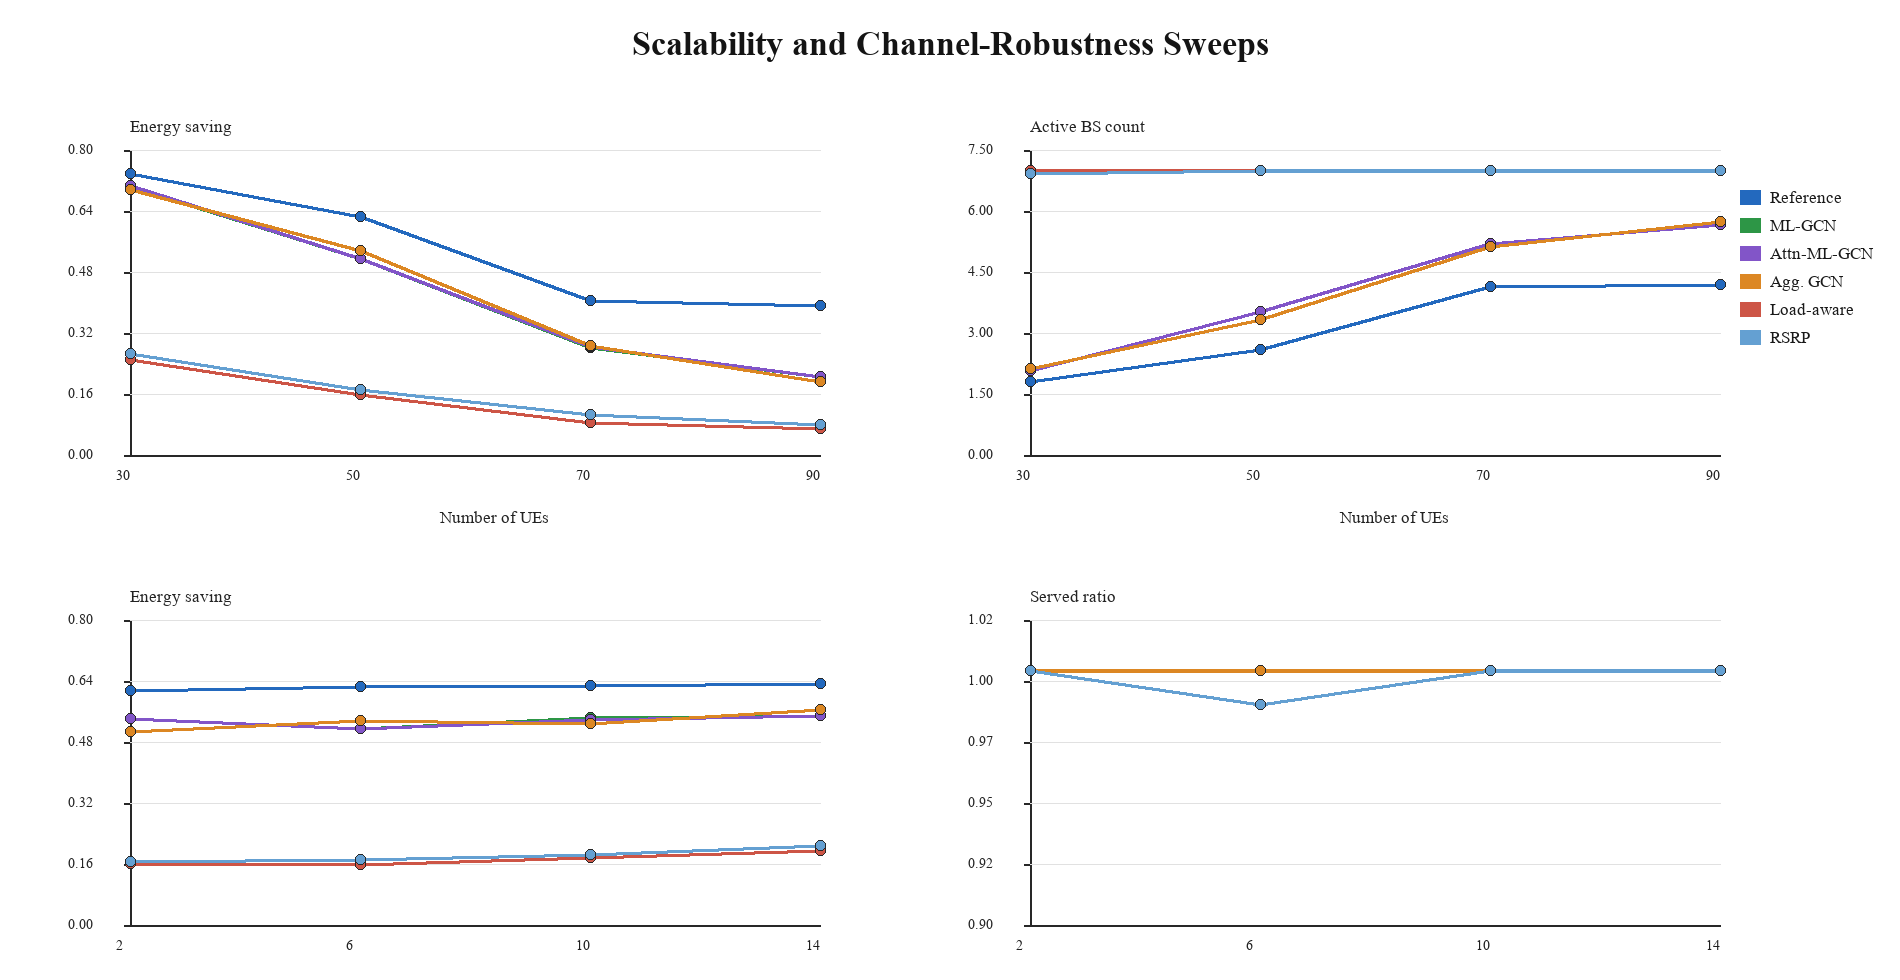
\includegraphics[width=\columnwidth]{figures/results/fig_results_scalability_robustness.png}
    \caption{Scalability and channel-robustness sweeps. Higher UE density
    reduces energy-saving opportunity and increases active BS count. Under the
    tested shadowing levels, the learned policies preserve service feasibility
    and remain more energy-efficient than conventional
    association rules.}
    \label{fig:results_scalability}
\end{figure}

\subsection{Layer Ablation}
Fig.~\ref{fig:results_ablation} reports layer ablation. Removing the load layer
has the largest leave-one-layer-out penalty: the energy saving decreases from
$55.4\%$ to $53.2\%$, and the active-BS count increases from 3.2 to 3.4. This
confirms that demand/load structure is relevant to deciding which BSs can
remain active without overload. Removing the association, interference, or
temporal layer also reduces energy saving, although with smaller penalties.

The single-layer comparison gives a complementary view. The interference layer
alone gives the largest single-layer improvement over the feature-only
baseline, while association, load, and temporal layers have smaller individual
effects but contribute jointly. Taken together, these two ablation views support the
modeling hypothesis that no single layer fully explains the energy-aware association
decision. The multilayer model benefits from preserving heterogeneous
dependencies before fusion.

\begin{figure}[!t]
    \centering
    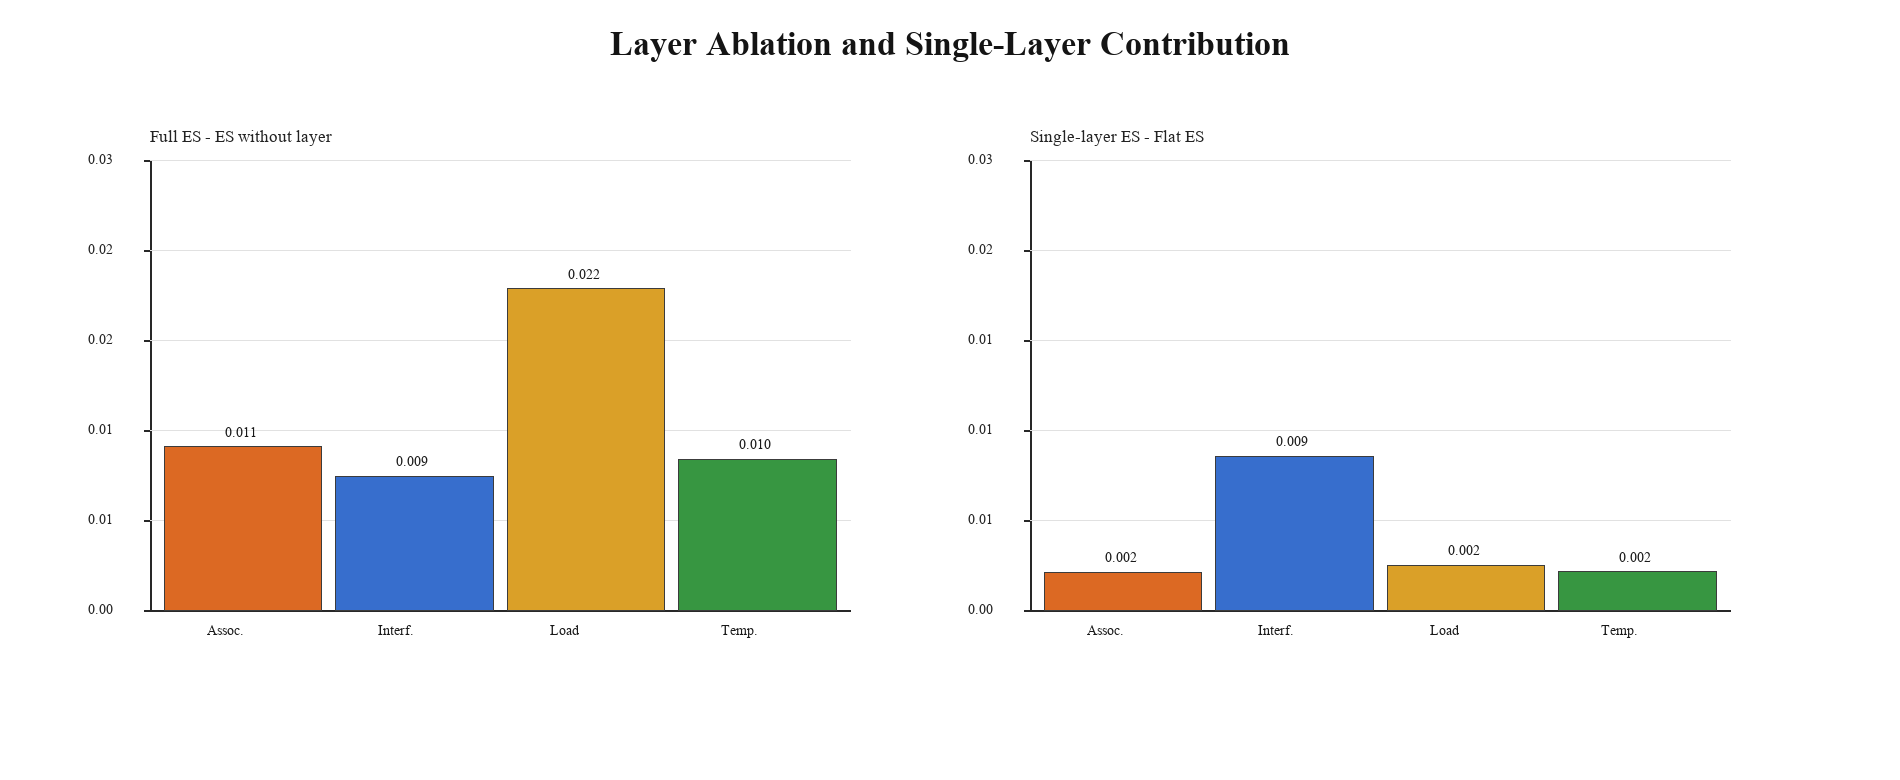
\includegraphics[width=\columnwidth]{figures/results/fig_results_layer_ablation.png}
    \caption{Layer ablation analysis. The load layer has the largest
    leave-one-layer-out effect, while the interference layer gives the largest
    single-layer gain over the feature-only baseline.}
    \label{fig:results_ablation}
\end{figure}

\subsection{Attention and Relation Dissimilarity}
Fig.~\ref{fig:results_attention} shows the learned attention distribution and
pairwise support-matrix dissimilarity. The attention model assigns comparable
weights to the four layers, with a mild preference for interference and load.
This explains why attention and fixed fusion perform similarly in the main
comparison: the current global attention mechanism does not strongly suppress
any layer. A more expressive snapshot-dependent attention mechanism may
differentiate layers more sharply under heterogeneous traffic regimes.

The dissimilarity heatmap shows that the temporal layer is the most distinct
from the association layer, while association and interference have moderate
overlap. The nonzero off-diagonal dissimilarities support the use of separate
relation layers rather than a single aggregated support. Even when attention
weights are nearly uniform, the layer-specific filters still process different
support matrices before fusion.

Layer dissimilarity and layer ablation indicate that the association,
interference, load, and temporal supports are not interchangeable projections
of the same graph. The control behavior therefore depends on which network
relations are preserved before learning. In the BS switch-off setting, the
controller acts on infrastructure states, while feasibility and stability are
determined by heterogeneous UE-UE relations.

\begin{figure}[!t]
    \centering
    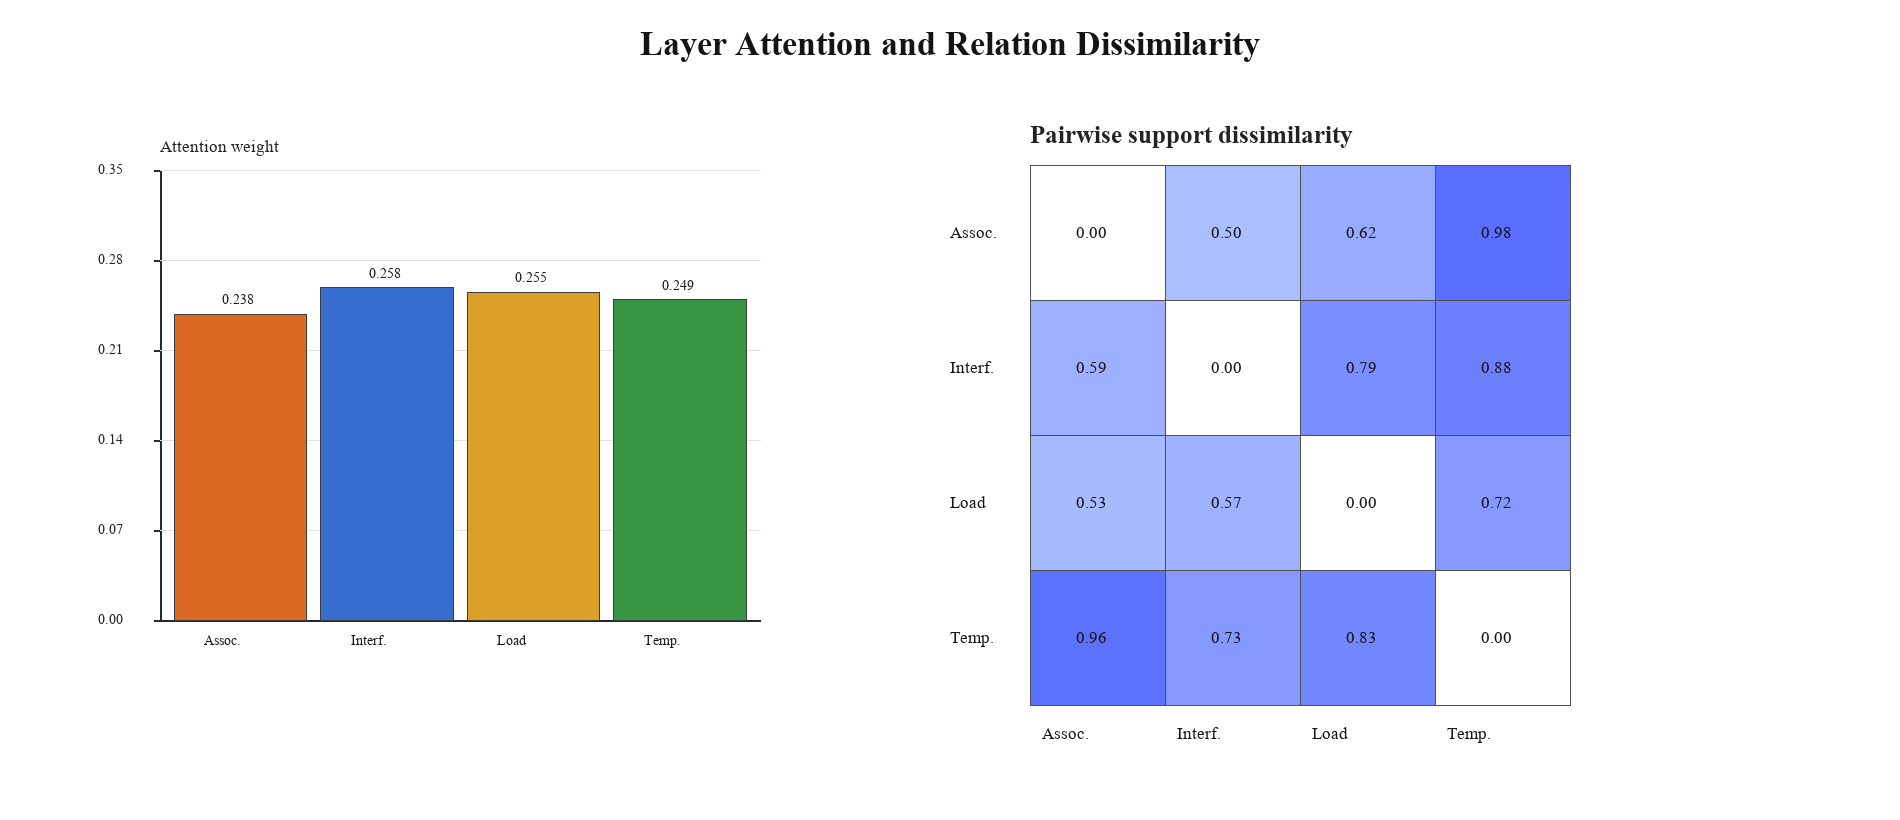
\includegraphics[width=\columnwidth]{figures/results/fig_results_attention_redundancy.png}
    \caption{Layer attention and relation dissimilarity. Attention weights are
    nearly balanced across relation layers, while the support matrices remain
    structurally distinct.}
    \label{fig:results_attention}
\end{figure}

\subsection{Discussion}
The experiments lead to four observations. First, association-only heuristics
do not compact the active-BS set and therefore provide limited energy savings
relative to sleep-control policies. Second, greedy sleep is an active-cell
pruning baseline for evaluating learned BS switch-off methods. Third,
switching cost changes the operational ranking because policies
with frequent active-cell transitions lose part of their static-energy benefit.
Fourth, the proposed method is formulated as a multilayer graph-control
framework with feasibility repair and active-cell stability, rather than as an
association-label classifier.

The results indicate that BS switch-off evaluation should include static
energy, switching-adjusted energy, served ratio, load feasibility, active-BS
count, and online decision latency. The proposed framework addresses these
criteria through the combination of multilayer representation learning,
active-cell selection, stability-aware pruning, and QoS/load repair. The
component ablation also indicates that the decision layer contributes
measurably to switching-aware performance, while the multilayer
representation provides a relation-aware and permutation-equivariant model of
the wireless dependencies.

\section{Conclusion}
This paper developed a switching-aware multilayer graph-learning framework for
energy-efficient user association and BS switch-off in dense wireless networks.
Each wireless snapshot was represented as a UE-level multilayer graph with
separate association, interference, load, and temporal relation layers. These
layers were processed by fixed-fusion and attention-weighted ML-GCN models,
and the learned association preferences were converted into feasible network
decisions by active-cell selection, score-guided pruning, stability-aware
pruning, and QoS/load repair.

The primary empirical finding is that the value of a BS switch-off policy depends on
whether active-cell transitions are counted. Greedy sleep control is a relevant
baseline, but in the simulation comparison the stability-aware ML-GCN improves
over it under both energy criteria. Stability-aware ML-GCN search achieves
$79.0\%$ static energy saving and $76.1\%$ switching-adjusted saving, compared
with $76.9\%$ and $68.3\%$ for greedy sleep, while maintaining served ratio
$1.0$. The improvement is supported by lower active-cell churn:
ML-GCN-stable-search reduces mean BS state changes from $2.50$ to $0.85$ per
snapshot. These results support
the proposed multilayer graph-control framework as an energy-efficient and
switching-aware approach to dense-network BS sleep control. Runtime
measurements showed that the stable learned policies have lower online latency
than greedy sleep and lower latency than finite active-cell
search. The component ablation indicates that, in the present implementation,
the stability-aware decision layer provides the largest contribution to
switching-adjusted performance, while the multilayer representation provides a
relation-aware and permutation-equivariant model for heterogeneous wireless
dependencies.

The study has several limitations. First, the evaluation is simulation based
and uses controlled channel, traffic, and power-model assumptions. These
assumptions support reproducible comparison, but they do not capture all
operational details of deployed radio access networks. Second, the finite
reference search is tractable for the considered BS scale and is used as a
bounded reference rather than as a scalable optimal solver. Third, the current
attention mechanism uses global layer weights; it does not yet adapt relation
importance on a snapshot-by-snapshot basis. Fourth, the stability-aware pruning
rule is a post-learning decision layer, so switching cost is not yet optimized
end-to-end inside the GNN training objective.

Future work will extend the framework in four directions. First, the
simulation environment should be expanded to include irregular BS deployments,
mobility traces, nonuniform traffic hotspots, and more detailed switching
delays and signaling costs. Second, adaptive attention and layer-selection
mechanisms should be developed so that relation importance can change with
traffic load, channel uncertainty, and topology. Third, switching cost and
feasibility constraints should be integrated more directly into training
through constrained learning, differentiable repair, or safe reinforcement
learning. Fourth, transfer across network sizes and operating regimes should be
evaluated so that models trained on one deployment can generalize to different
densities, bandwidths, and service requirements. These extensions would move
the proposed switching-aware multilayer graph framework closer to practical
energy-efficient control in future intelligent wireless networks.

\section*{Data and Code Availability}
The source code, simulation configurations, generated result files, MATLAB
figure scripts, and manuscript assets used in this study are publicly available
at \url{https://github.com/kazim01011/multilayer-ua-energy}. The repository
contains the simulator, multilayer graph construction routines, learning
models, baseline policies, reproducibility scripts, and aggregate CSV outputs
used to generate the reported tables and figures.

\bibliographystyle{IEEEtran}
\bibliography{references}
\end{document}
